\section{Unstructured \p\ Networks}
\label{section:unstructured}

In this section, we present algorithms that tackle the topology mismatch
problem in unstructured \p\ networks. We classify them based on their
use of the overlay structure, their message forwarding scheme 
for peer communication and the techniques they use for detecting
proximity.

\subsection{Algorithms for Unstructured Architectures}

% TODO: READ A Near-Optimal Algorithm Attacking the Topology Mismatch Problem in Unstructured Peer-to-Peer Networks)

% BROADCAST OPTIMIZATION

%%%%%%%%%%%%%%%%%%%%%%%%%%%%%%%%%%%%%%%%%%%%%%%%%%%%%%%%%%%%%%%%%%%%%%%%%%%%%%%%
% \subsubsection{Improving search in peer-to-peer networks}

% \begin{figure}[ht]
% \centering
% \subfigure[Iterative deepening with three levels.] {
%   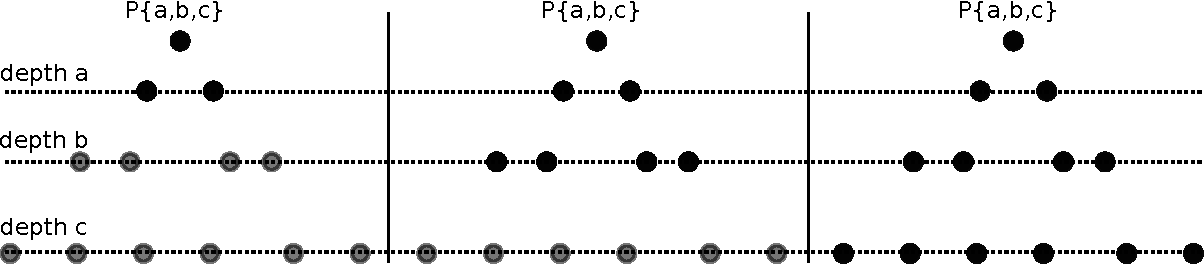
\includegraphics[scale=0.4]{img/algorithms/iterative_deepening}
%   \label{figure:dbfs:iterdeep}
% }\qquad\qquad
% \subfigure[Directed BFS.] {
%   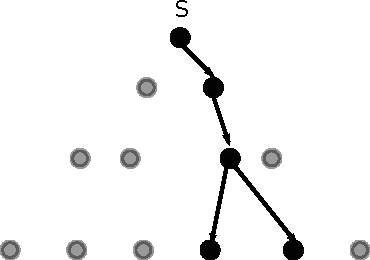
\includegraphics[scale=0.4]{img/algorithms/directed_bfs}
%   \label{figure:dbfs:dbfs}
% }\qquad\qquad
% \subfigure[Local indices with radius size equal to $2$.] {
%   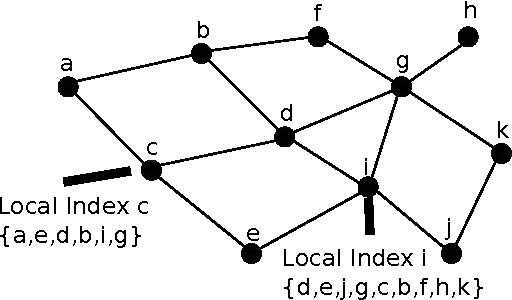
\includegraphics[scale=0.4]{img/algorithms/local_indices}
%   \label{figure:dbfs:localindx}
% }
% \caption{Improving search in P2P networks}
% \label{figure:dbfs}
% \end{figure}

To improve over {\sl Gnutella}'s ``blind flooding'' approach,
\cite{YG-M2002} proposed a practical and easy to implement solution 
weaved around three different message forwarding methods, namely
\emph{iterative deepening}, \emph{directed BFS} and \emph{local indices}.

In \emph{iterative deepening}, 
%(see Figure~\ref{figure:dbfs:iterdeep})
the search is
performed on a BFS tree with multiple preset depths. 
The depth limit is iteratively increased by the source node for each query, 
based on the quality of the results. 
The source node may issue a new request with increased depth limit
that will trigger the nodes at the last visited depth level to resume the
search thus avoiding restart of the entire search process and consequently 
reducing the load on the nodes of the upper levels of the tree. 
Its major drawback is the delay between successive iterations, as the
source-node has to examine the results at each attempt before deciding to
either quit or ``unfreeze'' the query.

The \emph{directed BFS}
tries to avoid the aforementioned delay by forwarding 
query messages only to a selected subset of available neighbors. The selection
criteria varies, from the number of results received or the distance (hops)
traveled to locate these results, to the bandwidth, or the
query load of the neighbor. That way, fewer nodes are visited but quality of
query responses is maintained, to a large degree, on the premise that the
selected heuristics can direct the search to the right path.
%
In \emph{local indices},
each node indexes data hosted by neighboring nodes within a radius of $r$ hops
and uses this local index to answer queries on behalf of other nodes.
That way, local indices,
greatly reduce the aggregate bandwidth usage of the network and 
improve query efficiency. However, updating such indices in 
the presence of frequent node joins/departures 
may introduce significant overhead should the radius is kept broad.
%%
Below, we outline how the techniques in~\cite{YG-M2002}
fare against the three major performance criteria 
of Section~\ref{section:background}.

\begin{center}
{\footnotesize
\begin{tabular}{rccc}
\multicolumn{1}{r}{} &
\multicolumn{1}{c}{\emph{Efficiency}} &
\multicolumn{1}{c}{\emph{Overhead}} &
\multicolumn{1}{c}{\emph{Scalability}}
\\
\cline{2-4}
\emph{Iterative Deepening} &
% needs recalculation in every iteration step
% extra delay imposed in a high churn environment that prohibits the algorithm
% to start from the last level of nodes and results in a restart of the whole
% process.
low &
% the process in not started from the beginning at each iteration step. For
% popular files this can substantially reduce overhead but for less popular
% ones, its performance might be uncertain due to the repeated restart of
% flooding
low &
% 
medium \\
\emph{Directed BFS} &
% Better time to satisfaction compared to iterative deepening
medium &
% Better quality and quicker results mean more aggregate bandwidth and
% processing power needs to be consumed since more nodes are involved (death
% spiral).
medium &
% BFS is Gnutella's non efficient communication method
medium \\
\emph{Local Indices} &
% efficiency is enhanced greatly since data pointers are replicated across the
% network
high &
% updating indices is a time and resource consuming process.
medium &
% the scalability is constrained by the indices update in a highly dynamic
% environment (high churn)
medium \\
\end{tabular}
}
\end{center}

%%%%%%%%%%%%%%%%%%%%%%%%%%%%%%%%%%%%%%%%%%%%%%%%%%%%%%%%%%%%%%%%%%%%%%%%%%%%%%%%
% \paragraph*{ \bf Delay Aware P2P System}
A \emph{delay--aware} \p\ system termed {\sl DAPS} 
was introduced in~\cite{ZL2005}.
{\sl DAPS}  seeks to attain reduced look-up times by dividing 
peer routing tables into several sectors of increasing delay. 
The source node that issues the query designates the delay 
boundary it may tolerate, providing so a \emph{pruning factor}.
In this context, user requests are forwarded only to 
nodes whose expected delay is less than or equal to the indicated boundary. 
{\sl DAPS} primarily focuses on user ``experience'' and deploys an
end-to-end delay monitoring mechanism that may enable
the clustering of routing tables. 
In a dynamic environment, the formation 
of very accurate such routing tables might be however an elusive goal.
%With the clustered
%routing tables and the loose organization of DAPS' overlay network it is
%considered by is be tween structured and unstructured.
%%
In terms of the three performance criteria, {\sl DAPS} stands as follows:
\begin{center}
{\footnotesize
\begin{tabular}{ccc}
\emph{Efficiency} & \emph{Overhead} & \emph{Scalability} \\
\hline
% Does not check for close by nodes, it just sorts the contents of a node's
% routing table.
% Also in a high churn environment a lot of time could be spend probing for
% distances, resorting routing tables and creating sectors. Moreover it just
% prunes distant neighbor
low &
% Sorting routing table entries is done locally so it is not affecting.
low &
%
medium
\end{tabular}
}
\end{center}

%%%%%%%%%%%%%%%%%%%%%%%%%%%%%%%%%%%%%%%%%%%%%%%%%%%%%%%%%%%%%%%%%%%%%%%%%%%%%%%%
% \subsubsection{Gia}
The key objective of the {\sl Gia} system~\cite{CRBLS2003} is 
to help alleviate the scalability omnipresent
in unstructured \p\ file-sharing systems.
At first, {\sl Gia} replaced {\sl Gnutella}'s blind flooding 
with random walks.
Although this adoption was 
a step in the right direction \cite{LCCLS2002},
issuing a single copy of the query within the network
effectively reduces the search scope and may negatively affect 
the success rate of the query in question.
To overcome this limitation, {\sl Gia} introduces
a token-based flow control mechanism 
that gradually redirects queries to nodes which are more
likely to answer. This flow control mechanism also helps prevent node
overloading as each peer ``announces'' the number of query requests it 
can handle, in terms of tokens, to its neighbors; to this end, 
peers only forward query requests to nodes that they previously
received tokens from. Further refinement to the search mechanism is the
support for \emph{one--hop replication} of pointers to content.
{\sl Gia} also acknowledges the heterogeneity in peer bandwidth,
processing power, disk speed, etc., of \p\ nodes and uses this
information when connecting nodes to each other.
By using a topology adaptation algorithm, 
{\sl Gia} places low capacity nodes within 
short proximity to peers with high performance features.
This topology adaptation algorithm is based on the metric 
each node maintains about its satisfaction --ranging between $0$ and $1$--
for the neighbors it finds itself associated with. 
Through message exchange, a peer can establish new connections 
or drop superseded ones in order to improve its satisfaction.
Despite the fact that {\sl Gia}'s topology adaptation algorithm 
that primarily focuses on the satisfaction of peers improves the network's
scalability, it falls short in addressing the mismatch problem
as considerations for the underlying network are not handled in explicit
terms \cite{LXLNZ2005}. Moreover it reduces the search scope, exhibits poor
performance in the worst case when matching data is not found quickly
\cite{PR2004,HJ2004} and can potentially build  disconnected topologies
\cite{MBL2006}.
%
In terms of the three stated criteria, {\sl Gia}'s approach is as follows:
\begin{center}
{\footnotesize
\begin{tabular}{ccc}
\emph{Efficiency} & \emph{Overhead} & \emph{Scalability} \\
\hline
% Reduces the search scope.
medium &
% Only one copy of the query is issued to the network.
% A token based flow control mechanism redirects queries to nodes that are most
% likely to fulfill them.
low &
% Even thought the low overhead scalability is reduced by the reducing of
% search scope.
medium
\end{tabular}
}
\end{center}

%%%%%%%%%%%%%%%%%%%%%%%%%%%%%%%%%%%%%%%%%%%%%%%%%%%%%%%%%%%%%%%%%%%%%%%%%%%%%%%%
% \subsubsection{Location-aware Topology Matching (LTM)}

\emph{Location-aware Topology Matching (LTM)} \cite{LLXNZ2004}
seeks to optimize an overlay \p\ structure based on the physical topology.
To achieve this, peers issue special messages called
\textit{TTL-detector}s whose \emph{TTL} values are $0$ or $1$;
in this regard, peers 
discover $1$- and $2$-hop neighbor sets, designated as $N$ and $N^2$
respectively, and proceed to compute communication costs.
Time-stamps are used to derive network latency measurements that are then used 
to improve the overlay network without sacrificing the search scope.
Each node compares the latency information
received from its direct neighbors;
peers with longer latencies are placed on a
\emph{will-cut} list where they remain for a certain period of time 
after which they are finally eliminated 
and are placed on the peer's \emph{cut-list}. 
Thus, low-productivity connections are dropped and replaced by 
more efficient ones, reducing the
latency on the overall network. 
Although \emph{LTM} improves the overall efficiency of
the \p\ network, it is unable to offer any warranty for 
effectively addressing the mismatch problem.
%
% TODO: SOME DISCUSSION
%
%\paragraph*{Low productive connection cutting}
%There are three cases for any peer $P$ who receives $d(i, S, v)$ multiple
% times:
%\begin{inparaenum}[\itshape i\upshape)]
%  \item $P$ receives both $d(i, S, 1)$ and $d(i, S, 0)$
%  \item $P$ receives multiple $d(i, S, 0)$s from different paths, and P
% randomly chooses to process one
%  \item $P$ receives one $d(i, S, 1)$ and multiple $d(i, S, 0)$s, and $P$
% processes $d(i, S, 1)$ and one randomly selected $d(i, S, 0)$
%\end{inparaenum}
%If the link with the largest cost is found and is a direct neighbor then the
% connection is put in a will-cut list and stays there for a certain period of
%time. If it is not, then it is handled by other peers. After that period,
%connections are cut and recorded to $P$'s cut-list.
%
%\paragraph*{Source probing}
%For a peer $P\in(N^2(S) - N(S))$ who receives only one $d(i, S, 0)$, the cost
% of $PS$ is obtained (with list look-up or probing). Then $P$ compares it with
%the cost from each hop and if $PS$ has the largest cost, $P$ will not keep this
%connection, while otherwise the connection will be created.
%
%\paragraph{}
%Supposing $n$ is the number of peers, $c_n$ is the average number of neighbors
% and $c_e$ is the average cost of logical links, then in the flooding-based
%search the traffic incurred by one query from an arbitrary peer in a
%peer-to-peer network is $O(n)$. As observed in the Gnutella network
%\cite{sripanidkulchai_gnutella_2001}, each peer issues $0.3$ queries per minute
%in average, thus the per minute traffic incurred by the network with $n$ peers
%is $O(n^2)$. Because each $d(i, S, v)$ has a TTL of $2$ in each source peer,
%the traffic for one time LTM optimization in all peers is at most $2nc_n^2c_e$.
%If each peer uses LTM $k$ times per minute, the total traffic incurred is
%$2knc_n^2c_e$. Simulation shows the best value for $k$ is $2$ or $3$ So, the
%traffic overhead caused by LTM to the network is $O(n)$.
%
%TTLj-detectors, with $j > 2$, would detect and break cycles with more than 4
% links. LTM though, does not use such detectors because detector-flood traffic
%would increase significantly, and cut links between two end-peers, could cause
%queries initiated by them to traverse a path much more expensive than the cost
%on the the cut link.
%
%\paragraph{}
%LTM disadvantages are
%\begin{inparaenum}[\itshape i\upshape)]
%  \item disagreement of measured delay due to unsynchronized clocks causes
% problems when deciding the cut positions, which can influence the network
%connectivity, and
%  \item the network delay metric mainly focuses on disabling the connections
% between peers physically far away without considering the shortcuts created by
%powerful peers.
%\end{inparaenum}
%
\emph{LTM} fares as follows regarding our three  criteria:
\begin{center}
{\footnotesize
\begin{tabular}{ccc}
\emph{Efficiency} & \emph{Overhead} & \emph{Scalability} \\
\hline
% Authors claim 75% reduction on traffic cost and about 65% reduction on query
% response time.
medium &
%
medium &
%
medium
\end{tabular}
}
\end{center}

%%%%%%%%%%%%%%%%%%%%%%%%%%%%%%%%%%%%%%%%%%%%%%%%%%%%%%%%%%%%%%%%%%%%%%%%%%%%%%%%
% \subsubsection{Distributed Cycle Minimization Protocol (DCMP)}
Another problem with topology unaware
systems is the duplication of messages due to cycles in the network graph.
Interestingly, such cycles appear even along the correct forwarding path.
\cite{ZKB2008} focuses on this exact deficiency of overlay networks and
introduces the \emph{Distributed Cycle Minimization Protocol
(DCMP)}, a dynamic, fully distributed method that removes cycles;
this is accomplished without sacrificing
overlay connectivity, resilience and other key properties of unstructured
\p\ architectures and by avoiding a hierarchical organization of peers. 
Once a cycle is detected in {\it DCMP}, the most powerful node in that cycle 
is elected as the \emph{Gate Peer} and the cycle is then broken in that place
that it will result in the minimization of the distance between the
\emph{Gate Peer} and all other nodes that are currently part of the cycle. 
This process is managed by using two specialized message types 
namely, \emph{Information Collection Message (ICM)} and \emph{Cut Message (CM)}. 
\emph{DCMP} bases its operation on messages whose travel is limited by an
imposed \emph{TTL} value (max set to $7$ for most cases). This inherently limits
the protocol in detecting cycles that span for more than \emph{TTL} nodes.
Even though cycle elimination does improve network performance, 
it cannot  directly contribute to the solution of the topology mismatch
problem, while its performance in a high traffic and churn environments and its
ability to retain important characteristics of a {\sl Gnutella}-like topology (i.e.,
like degree distribution, average peer distance, diameter e.t.c.) has been
doubted~\cite{CSG2010}. 
On the other hand, even though some of the overhead
saved by the duplicate message reduction is spent to control the cycle cutting
mechanism, it is reported that it does a lot better in that area
due to its ``lazy'' broadcasting of control messages, as opposed to, for example,
LTM's periodic approach \cite{ZKB2008}.
%
%\begin{figure}
%\centering
%  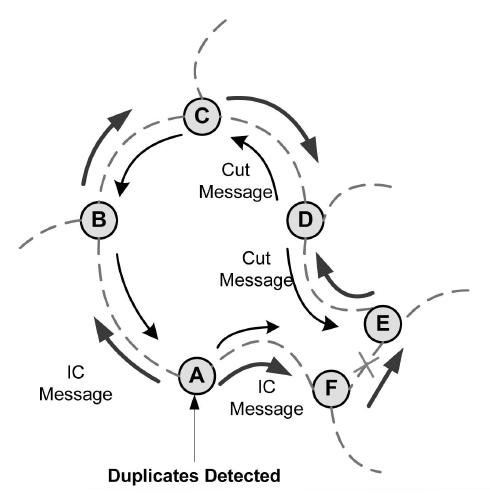
\includegraphics[scale=0.4]{img/dcmp.jpeg}
%\caption{Cycle elimination methods in DCMP}
%\label{figure:dcmp}
%\end{figure}
%
% TODO: SOME DISCUSSION
%Actually, the duplicate packet problem seems to hurt more the active nodes;
%those with higher capacities and bandwidth that contribute the most to the
%network.
The expected \emph{DCMP} behavior as far as our three criteria is:
%
\begin{center}
{\footnotesize
\begin{tabular}{ccc}
\emph{Efficiency} & \emph{Overhead} & \emph{Scalability} \\
\hline
% It returns more result than LTM according to experiments in
% \cite{ZKB2008}
medium &
% Duplicates are an important fraction of the redundant overhead imposed by
% topology mismatch and thus DCMP minimizes this as possible.
% It is reported though that still stays for example one to two orders of
% magnitude less than LTM due to its ``lazy'' broadcasting of control messages
% (as opposed to LTM's periodic approach) \cite{ZKB2008}.
low &
% fully distributed method
high
\end{tabular}
}
\end{center}

%       CACHING

%%%%%%%%%%%%%%%%%%%%%%%%%%%%%%%%%%%%%%%%%%%%%%%%%%%%%%%%%%%%%%%%%%%%%%%%%%%%%%%%
% \subsubsection{Replication Strategies in Unstructured Peer-to-Peer Networks}

In \cite{CS2002} and \cite{LCCLS2002}, replication is used as a way to improve
inefficient blind search. The observation is that as the number of replicas
increases in the network, it would be relatively easy to locate items even if
search is random. Concretely, three three approaches for replication allocation
are discussed: \emph{uniform}, \emph{proportional}, and
\emph{square-root replication}.

In the uniform model, all objects are replicated without taking into account
the query distribution,
while in the proportional, objects are replicated analogously to their query
rate, so that frequently queried items can be found more often. Experimental
outcomes indicate that the uniform allocation minimizes the maximum search
length and so it can reduce the time spent on unsuccessful searches. The
proportional strategy effectively decreases the search time for popular items,
but suffers when needing to locate the rare entities. When it comes to expected
successful search size, it is the same for for both uniform and proportional
models and any approach in between to always behave much better. Finally, the
square-root model is an attempt to find the golden ratio between uniform and
proportional allocation models. It suggests setting the number of object
replicas to the square root of the searching rate for an object\footnote{An
interesting application of the square-root principle has also been explored
in the context of topology reconstruction, by ensuring node degree to be
proportional to the square-root of its content popularity \cite{C2005}.}.
Theory in \cite{CS2002} suggest that square-root minimizes the expected search size on
successful queries, claim that is supported by simulations \cite{LCCLS2002}.  

In \cite{LCCLS2002}, a \emph{k-walker} query algorithm is presented and shown
that using it along side square-root allocation results in performance similar to
{\sl Gnutella}'s query flooding method but incurring up to two
orders of magnitude less network traffic. Also checks three strategies for
replica placement, namely \emph{owner replication} where an object is replicated
at the requesting node, \emph{path replication} that caches the object along the
path from the requesting to the providing node and \emph{random replication}
where the replication is taking place randomly on visited nodes. Observations in
this work are not directly applicable to structured DHTs, because it is assumed
that the lookup time for an object depends only on the number of replicas and
not the placement strategy \cite{RS2004}.

%%
%% SOME EXTRA DISCUSSION TAKEN FROM
%% IRM: Integrated File Replication and Consistency Maintenance in P2P Systems
%% 
%% Lv et al. [21] and Cohen and
%% Shenker [22] showed that replicating objects proportionally
%% to their popularity achieves optimal load balance but has
%% varied search latency, while uniform replication has the
%% same average search latency for all files but causes load
%% imbalance. Square-Root replication method replicating files
%% proportionally to the square root of their popularity is such
%% that both average search size and capacity utilization rate
%% vary per object, but the variance in utilization is consider-
%% ably smaller than with uniform replication, and the variance
%% in average search size is considerably smaller than with
%% proportional replication.
%%

The table below outlines how the three allocation approaches fare:
%%
\begin{center}
{\footnotesize
\begin{tabular}{rccc}
\multicolumn{1}{r}{} &
\multicolumn{1}{c}{\emph{Efficiency}} &
\multicolumn{1}{c}{\emph{Overhead}} &
\multicolumn{1}{c}{\emph{Scalability}}
\\
\cline{2-4}
\emph{Uniform Replication} &
% Proportional and Uniform are the worst “reasonable” strategies
low &
% When item is created, replicate its key in a fixed number of hosts.
low &
%
medium \\
\emph{Proportional Replication} &
% Proportional and Uniform are the worst “reasonable” strategies
low &
% for each query, replicate the key in a fixed number of hosts (need to know or
% estimate the query rate)
medium &
%
low \\
\emph{Square Root Replication Allocation} &
% All (strictly) in-between strategies are (strictly) better than Uniform and
% Proportional - replication theory
medium &
% Assuming that each query keeps track of the search size then each time a query
% is finished the object is copied to a number of sites proportional to the
% number of probes that the search required.
medium &
% e.g. path replication is easy to scale, just detect the path along which the
% query ultimately got fulfilled
medium \\
\end{tabular}
}
\end{center}

%%%%%%%%%%%%%%%%%%%%%%%%%%%%%%%%%%%%%%%%%%%%%%%%%%%%%%%%%%%%%%%%%%%%%%%%%%%%%%%%
% \subsubsection{Tracing a large-scale Peer to Peer System: an hour in the life
% of Gnutella}
% TODO: This looks better as an analysis for the unstructured networks in
% general and specifically for caching, so it doesn't seem to contribute any
% new approach.... At least we do not present anything here. Maybe we need to
% revisit the paper itself once more
% \cite{Markatos02} analyses Gnutella network traffic traces and by concluding
% there is locality among query requests, proposes a caching algorithm that tries
% to exploit these findings . The analysis of the trace data reveals other
% important facts about the structure of the Gnutella network and the query data.
% One significant observation is that the geographic locations of clients do not
% have a correlation with the number of query requests they receive. This is an
% obvious result of the topology mismatch problem caused by the overlay structure
% of the Gnutella network. Gnutella's traffic is observed to be bursty both for
% query requests and query responses, even in longer intervals. It is observed
% that a peer receives 50 query messages per second on average! Moreover nine out
% of ten queries do not generate any response due to the inefficient design of
% the Gnutella network. When developing a caching system to exploit locality,
% applying an approach similar to web caching does not fit well with P2P systems.
% Caches in P2P systems not only have to consider the query string, but also
% the TTL value, the source of the query, and the time of the query as well.  In
% general, even though optimum caching is hard to achieve, it is reported that
% it improves the overall performance of the Gnutella network.

% \begin{center}
% \begin{tabular}{ccc}
% \emph{Efficiency} & \emph{Overhead} & \emph{Scalability} \\
% \hline
%
% ? &
%
% ? &
%
% ?
% \end{tabular}
% \end{center}


%       OVERLAY OPTIMIZATION

%%%%%%%%%%%%%%%%%%%%%%%%%%%%%%%%%%%%%%%%%%%%%%%%%%%%%%%%%%%%%%%%%%%%%%%%%%%%%%%%
% \subsubsection{Narada}

% \begin{figure}[ht]
% \centering
% \subfigure[Underlying network with edge costs.] {
%   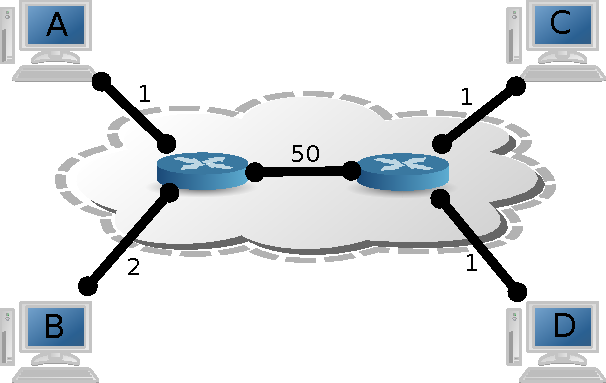
\includegraphics[scale=0.4]{img/algorithms/narada}
%   \label{figure:narada:underlying}
% }\qquad\qquad
% \subfigure[Peer A sends a message to the rest using regular broadcast.] {
%   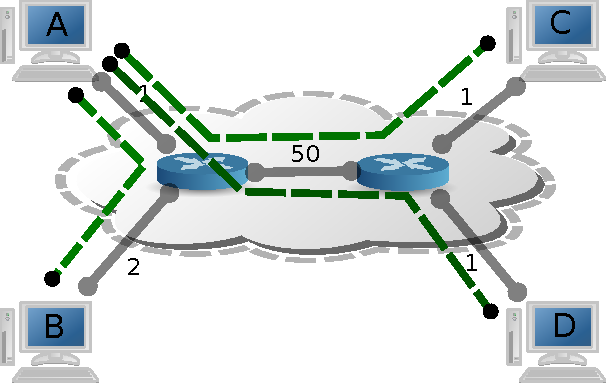
\includegraphics[scale=0.4]{img/algorithms/narada2}
%   \label{figure:narada:regu}
% }\qquad\qquad
% \subfigure[Peer A sends a message to the rest using end system multicast.] {
%   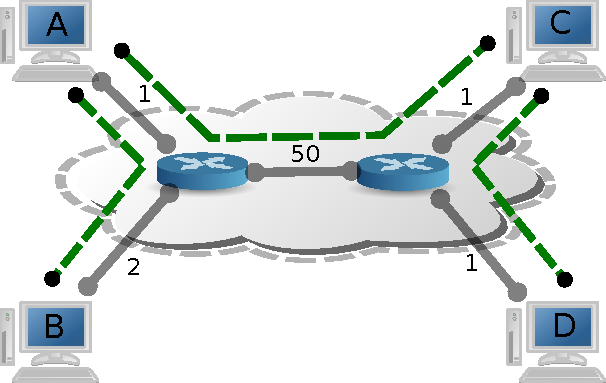
\includegraphics[scale=0.4]{img/algorithms/narada3}
%   \label{figure:narada:multicast}
% }
% \caption{A visualization of the Narada protocol.}
% \label{figure:narada}
% \end{figure}

{\sl Narada}~\cite{CRZ2000,CRSZ2001,CRSZ2002} is a generic
protocol for creating self-adapting overlay networks capable of 
application-layer multicast communications without requiring IP multicast
infrastructure at the network layer.
Although IP--multicast would present a choice in implementing
{\sl Narada}, it is in general considered that it violates the 
stateless design of the current Internet.
Despite the fact the {\sl Narada} was not designed as \p\ system per se,
it was the first (along with \emph{Scattercast} \cite{C2000}) to consider the
feasibility of overlay-based, application-layer services over the Internet while
taking into account bandwidth and latency properties of the underlying physical
infrastructure. In the context of this work, the inefficiency caused by the
topology mismatch is attempted to be tackled by building a highly connected
graph, termed \emph{mesh},
with each source featuring its own minimum spanning tree. A gossip-protocol was
deployed for the creation of these spanning trees~\cite{LYL2008}.
%as shown in Figure~\ref{figure:narada}.
The graph and trees are dynamically updated as nodes keep joining 
or departing the network. The protocol aims to ease the physical link stress,
the overall resource usage as well as the relative delay among end-systems. 
Unfortunately, the main limitation for {\sl Narada} is that 
although it works reasonably well for small groups, 
it does not scale well for larger networks. 
Hence, it is not a suitable choice for potentially large \p\ networks:
%%
\begin{center}
{\footnotesize
\begin{tabular}{ccc}
\emph{Efficiency} & \emph{Overhead} & \emph{Scalability} \\
\hline
%
medium &
% The overhead of Narada is proportional to the multicast group size
high &
% Maintaining the mesh for large multicast groups is expensive.
low
\end{tabular}
}
\end{center}

%%%%%%%%%%%%%%%%%%%%%%%%%%%%%%%%%%%%%%%%%%%%%%%%%%%%%%%%%%%%%%%%%%%%%%%%%%%%%%%%
% \subsubsection{Adaptive Overlay Topology Optimization (AOTO)}

Along with {\sl Narada}, the \emph{Adaptive Overlay Topology 
Optimization (AOTO)} \cite{LZXN2003} is one of the first attempts to address the
topology mismatch problem. \emph{AOTO} is a distributed algorithm that seeks to
optimize the usage of the underlying physical resources and operates in
$2$ phases:
\emph{Selective Flooding} and \emph{Active Topology}.
In \emph{Selective Flooding}, a minimum spanning tree is built for each peer and
its immediate neighbors so that queries do not flood the entire network and at
the same time preventing their search scope from shrinking. This way some
neighbors become non--flooding. During \emph{Active Topology}, each peer
replaces independently such non--flooding neighbors, with closer nodes as an attempt
to revise the overlay links so that they can reflect more closely the physical
network topology. Picking a replacement out of these non-flooding
neighbors follows a random policy called \emph{Randomized AT} algorithm.
To accomplish the above actions, a peer has to keep track of 
its communication costs with all its neighbors (e.g., network delays)
as well as the costs between any pair of neighbors. The \emph{randomized AT}
algorithm is applied by a source peer
every time its neighbor list is updated or an updated neighbor cost 
table is received.
%%
%\paragraph*{Selective Flooding (SF)}
%
% TODO: I DON'T REMEMBER WHY THE FOLLOWING IS MENTIONING LTM WHICH IS ANOTHER
%       ALGORITHM. MAYBE THIS CAN BE USED AS A PART OF DISCUSSION AND/OR
%       COMPARISON OF AOTO AND LTM
% TODO: EDIT: LTM SEEMS A MISTAKE HERE BETTER NOT USE IT FOR DISCUSSION (THIS
%             IS AOTO)
%LTM's SF effectiveness has be proven to be detached from the different physical
% or overlay topologies. On the other hand, SF is more effective with large
%number of logical neighbors. It can reach an average optimization rate of 87.4
%percent on a logical topology with an average of 30 logical neighbors.
%
%\paragraph*{Active Topology (AT)}
%
%Different numbers of average logical neighbors has little to do with the
% effectiveness of AT. If the source has $n$ non-flooding peers, there are $n$
%potential neighbor replacements. The overhead to exhaust all $n$ possible
%replacements can be high, so in practice, after each replacement the source
%peer can decide whether it needs to find another candidate peer. This is done
%by computing the cost improvement ratio greater than some predefined
%termination threshold. The larger the threshold, the slower, in the number of
%optimization steps, the reduction of the normalized average distance. As a
%whole the average response time is significantly reduced when more optimization
%steps taken.
%%
\emph{AOTO}'s performance regarding the three criteria is as follows:
%%
\begin{center}
{\footnotesize
\begin{tabular}{ccc}
\emph{Efficiency} & \emph{Overhead} & \emph{Scalability} \\
\hline
%
medium &
% tracking of communication costs to all peer's neighbors as well as between
% any pair of neighbors. Whenever a new neighbor cost table is received or
% there is a change of neighbors, the source peer has to re-calculate the
% multicast tree and apply the randomized AT algorithm.
high &
% needs global knowledge
medium
\end{tabular}
}
\end{center}

%%%%%%%%%%%%%%%%%%%%%%%%%%%%%%%%%%%%%%%%%%%%%%%%%%%%%%%%%%%%%%%%%%%%%%%%%%%%%%%%
% \subsubsection{Adaptive Connection Establishment (ACE)}
The \emph{Adaptive Connection Establishment (ACE)} 
approach~\cite{LZXN2004} uses the network delay as a metric 
to estimate the costs between nodes. Each peer computes the costs to its
logical one-hop neighbors and forms a \emph{neighbor cost table (NCT)} 
using a special routing message type. 
Any pair of neighboring peers exchange their \emph{NCT}s 
and so a minimal overlay topology can be formed. Based on the obtained
\emph{NCT}s a minimum spanning tree for each peer and its one-hop neighbors is
created. Finally, neighbors located physically far away 
are replaced by physically-closer counterparts. 
In particular, a peer $S$ iteratively probes the distance $d$ between
itself and every of its non-flooding neighbor nodes $G$ as well as
the distance between $S$ and $G$'s neighbors designated as $H$.
If $d_{SG} > d_{SH}$, then link $SG$ is replaced by link $SH$. If, on the other
hand, $d_{SG} < d_{SH}$ then also $d_{GH}$ and then we have the following
options. Either $d_{SH} < d_{GH}$ in which case link $SH$ is kept or
$d_{SH} > d_{GH}$ in which case $S$ will keep probing other $G$'s direct
neighbors.
%
The above optimization is conducted within $1$-neighbor
closure using as base, a peer and checking all its direct neighbors.
Evidently the scope of such an operation could be extended.
Should  a larger scope be used, a better topology matching can be obtained 
at a greater computational overhead.
%
% TODO: SOME DISCUSSION
%
%Simulations in \cite{liu_acesims_2004} show that the average scope of each
% query to cover the same scope of nodes is reduced by about 65 percent without
%losing any autonomy feature, while the average response time can be reduced by
%35 percent. Larger diameter topologies lead to better topology optimization
%rate but also to higher communication and computation overhead. It was also
%found that it is more effective in higher connectivity dense topologies.
%Compared to LTM, it comes short of convergence speed. In
%\cite{ni_mismatch_2004} shows reduction of both total traffic (90 percent) and
%response time (80 percent) to message queries without shrinking the search
%scope.Last but
%not least, it is concluded that work must be done on incorporating a more
%sophisticated selection policy for candidate non-flooding peers.
%

%In \emph{Adaptive Connection Establishment (ACE)} \cite{LZXN2004}, the
%authors extend the idea of AOTO by introducing optimizations based on the
%depths of the minimum spanning trees. But since the network delay is not
%always a reliable estimation method to detect the physical location of peers,
%the algorithm still suffers from the discrepancies caused by mis-located nodes.
%%
%%
\begin{center}
{\footnotesize
\begin{tabular}{ccc}
\emph{Efficiency} & \emph{Overhead} & \emph{Scalability} \\
\hline
% compared to LTM it has slow convergence speed because of the information
% exchange among each peer and all its neighbors.
medium &
% A little bit better that AOTO since the computation here is done within a
% certain diameter from the source peer
medium &
% Larger diameter topologies lead to better topology optimization
% rate but also to higher communication and computation overhead.
medium
\end{tabular}
}
\end{center}

%%%%%%%%%%%%%%%%%%%%%%%%%%%%%%%%%%%%%%%%%%%%%%%%%%%%%%%%%%%%%%%%%%%%%%%%%%%%%%%%
% \subsubsection{Scalable Bipartite Overlay (SBO)}

The \emph{Scalable Bipartite Overlay (SBO)}~\cite{LXN2007} 
reduces the overhead of creating
and maintaining a minimum spanning tree 
by randomly dividing the nodes into
two groups --\emph{red}s and \emph{white}s-- 
and assigning different tasks to the two groups.
When a peer joins the network, it is randomly assigned with an initial
color (red or white).
Then the network bootstrap host node furnishes the joining peer with a list
of active peers along with their color information. 
The joining peer uses this list to 
establish connections to differently colored peers. 
In this regard, all peers form a bipartite overlay. 
Using the network delay as metric, white-peers 
measure distances from red counterparts
and report the encountered red neighbors.
Having information on all their $2$-hop neighbors 
($N^2$)
red-peers create minimum spanning trees for the neighbors in question and
assign efficient $2$-hop forwarding paths. This process can render a white-peer
$E$ non--forwarding neighbor of the red-peer $P$. Direct neighbor
replacement is a process conducted by $E$ in order to replace $P$ with a
$P' \in N^2(P)$ as its new neighbor. This adaptation tackles the
topology mismatch problem by reducing message duplication and shorten response
times caused by the problem identified as \emph{Revisit Not known (RN)}. RN is
the situation when a node is visited some times as a relay stop before it is
visited as an overlay peer, thus creating duplicate unnecessary messages to the
network and delaying query responses.
Even though this attempt is based on a simple and elegant solution it is
reported to not guarantee performance in terms of average communication delay
or search scope \cite{HLH2009}.
%
% TODO: SOME DISCUSSION
%
%In a static environment LTM may reduce traffic cost by around 80 to 85 percent
% while SBO reduces traffic cost between 85 and 90 percent. However, LTM  is
%proved to converge in around 2-3 steps while SBO needs 4-5 steps. Moreover LTM
%reduces response time by more than 60 percent in 3 steps while SBO needs 8. In
%a dynamic environment (10 minute average peer lifetime, 0.3 queries/sec by each
%peer) SBO and LTM reduce the average traffic cost per query (including the
%overhead due to the optimization steps) by 85 and 80 percent, respectively.
%Moreover LTM reduces the response time per query to 30 percent while SBO to 35
%percent.
%
% THE LINES BELOW NEED REWORDING
% ==============================
% \cite{LXN2007} Based on the above discussions, we can see the major
% advantages of using a bipartite overlay. First, the operation
% overhead is reduced. In ACE, every peer is required to
% probe the neighbor distance and compute the MST, whereas
% in SBO, white peers do the probing and red peers do the
% computing. Second, SBO extends ACE into two-hop
% neighbors, without additional information exchange
%
%\cite{ni_mismatch_2004} shows SBO, achieves approximately 85 percent reduction
% on traffic cost and about 60 percent reduction on query response time.
In regards to the three stated criteria, \emph{SBO} behaves as follows:
\begin{center}
{\footnotesize
\begin{tabular}{ccc}
\emph{Efficiency} & \emph{Overhead} & \emph{Scalability} \\
\hline
% SBO reduces traffic cost between 85 and 90 percent
high &
% compared to LTM it has slower convergence speed thus incurs more, total,
% overhead.
medium &
%
medium
\end{tabular}
}
\end{center}

%%%%%%%%%%%%%%%%%%%%%%%%%%%%%%%%%%%%%%%%%%%%%%%%%%%%%%%%%%%%%%%%%%%%%%%%%%%%%%%%
% \subsubsection{Two-Hop-Away Neighbor Comparison and Selection (THANCS)}

The distributed heuristic termed 
\emph{Two-Hop-Away Neighbor Comparison and Selection (THANCS)}~\cite{LNXE2005,L2008}
attempts to minimize overlay hop costs.
\emph{THANCS} is essentially a \emph{local search method} as it aims 
to find a locally optimum solution by exploiting knowledge within 
a $2$-hop radius. The algorithm consists of two main components:
\emph{piggybacking neighbor distance on queries} and
\emph{neighbor comparison and selection}.

The \emph{piggybacking component} requires peers 
to probe immediate neighbors using delay distance measurements 
and store this information locally. 
The algorithm introduces a special query message type, 
the \emph{Piggy Message (PM)} which includes information about 
the neighbor identification (\emph{IP}) and measured distance ($d$). PMs are
piggybacked to normal
{\sl Gnutella} messages. 
When a node $P$ receives a query from $Q$, it constructs a
$PM_{PQ}$, piggybacks it to the query and forwards it to $P$'s neighbors. 
As soon as a neighbor detaches a received $PM_{PQ}$, records the distance 
$d_{PQ}$ and processes the query.
% When the neighbors receive it they detach the $PM_{PQ}$, 
% record the distance $d_{PQ}$ and process the query normaly. 
Selection of which incoming queries
should be piggybacked with a \emph{PM} is determined using either a
% proposed by either
\emph{pure probability-based (PPB)} or a \emph{new neighbor triggered (NNT)}
policy.


The \emph{neighbor comparison and selection} component defines that a peer $S$
probes all his $2$-hops away neighbors (a set denoted as $ N^2(S)$) not probed
thus far. Let $P$ be a $1$-hop distance neighbor of $S$, and $Q$ be a probed
peer by $S$. When $S$ receives a message piggybacked with message $PM_{PQ}$, 
the following $2$ cases are identified:

\begin{enumerate}
  \item If $Q$ is already a direct neighbor of $S$ then we check 
	the distances $d_{SQ}$, $d_{SP}$ and $d_{PQ}$. 
	If either $d_{SQ}$ or $d_{SP}$ is the longest, then the longest
  	link will be placed in a \emph{will-cut} list\footnote{A peer will not send or
  	forward queries to connections in its will-cut list but will preserve them
  	for some time in order not to effect ongoing response messages travelling the
  	inverse path.}. 
	If $d_{PQ}$ is the longest, then nothing is done by $S$; being
  	fully distributed, neighbor comparison and selection process, will have the
  	opportunity to handle $PQ$ link when initiated by peers $P$ or $Q$.

  \item If $Q$ is strictly a $2$-hop neighbor of $S$ and have never probed $Q$
  	in the past, stores distance $d_{SQ}$ and checks 
	distances $d_{SQ}$, $d_{SP}$ and $d_{PQ}$.
  	If $d_{SQ}$ is the longest, $S$ will not create link $SQ$. If $d_{SP}$ is the
  	longest, $SQ$ will be created and $SP$ will be put into the will-cut list.
  	If $PQ$ is the longest, links $SP$ and $SQ$ will be preserved expecting that
  	$P$ or $Q$ will disconnect $PQ$ later.
\end{enumerate}

%
% TODO: SOME DISCUSSION
%
% \begin{inparaenum}[\itshape i\upshape)]
%   \item is completely distributed and needs no global knowledge,
%   \item presents trivial overhead compared to the query cost savings
%   \item its convergent speed of the algorithm is fast enough (faster than
% minimum spanning tree approaches) so that is effective to dynamic
% environments, and
%   \item does not shrink the search scope.
% \end{inparaenum}
%
%In a static environment THANCS has been proven to be effective; optimizing 45
% percent out of the 60 percent of mismatched paths, constructing a nearly
%optimal overlay. This leads to a 60 percent reduction in traffic cost as well
%as a 40 percent decrease in query response time. In dynamic environments
%(Gnutella 0.6/Limewire super-peer-like and Ion flat-like), THANCS saves up to
%70 percent of the traffic cost in the super-peer topology and 55 percent for
%the flat one. Average response time is also decreased by 60 and 45 percent,
%respectively. Generally, THANCS has similar performance to LTM, without needing
%synchronization. SBO, incurring half the  overhead of AOTO, reduces the traffic
%cost the most, while THANCS has lower response time and converges faster than
%SBO. THANCS is, thus, more suitable for a more dynamic environment. In
%addition, THANCS is easy to implement and its operation overhead is trivial,
%compared with the other three approaches. This design, however, has the
%limitation of not being easily extend to also support non-flooding-based
%systems.

As discussed above, \emph{THANCS} is fully distributed and needs only minimum knowledge
of, at most, a $2$-hop distant peers. This features renders 
the method a good candidate for large overlay networks.
Also its topology adaptation helps construct a well fit overlay
with respect to the underlying network--at least with respect to network
distances. In addition, will-cut list and distance caches (which store already
probed peers) minimize the unnecessary messages for the network maintenance.
%%
\emph{THANCS} reportedly improves brodcast performance the extent of which, though,
depends on the underlying network since \emph{THANCS} does not provide the
performance guarantee for the improvement of any given overlay topology~\cite{HLY2010}.

%%%%%%%%%%%%%%%%%%%%%%
\begin{center}
{\footnotesize
\begin{tabular}{ccc}
\emph{Efficiency} & \emph{Overhead} & \emph{Scalability} \\
\hline
% 
medium &
% trivial overhead compared to the query cost savings and its convergent speed
% is faster than minimum spanning tree approaches so less overall overhead cost.
low &
% completely distributed and needs no global knowledge,
high
\end{tabular}
}
\end{center}

%%%%%%%%%%%%%%%%%%%%%%%%%%%%%%%%%%%%%%%%%%%%%%%%%%%%%%%%%%%%%%%%%%%%%%%%%%%%%%%%
The \emph{Hops Adaptive Neighbor Discovery (HAND)} algorithm~\cite{CLZHC2006}
uses a fully-distributed triple--hop adjustment strategy, applied to a network
graph $G$ in order to create an optimal graph $G^{*}$, free of the implications
of topology mismatch. This optimality is attained if all peer hop 
sequences $(v_1, v_2, \ldots, v_k)$ of $G$ exist in $G^{*}$ and are in the same
order. The latter indicates that in practice triple sequences $(v_1, v_2, v_3)$
are used. A mismatch is detected as follows: should we want to verify
a sequence, say $v_2-v_1-v_3$, two probing messages are dispatched from $v_1$ to
$v_2$ and $v_3$ and yield delays of $x$ and $z$ respectively.
%
When the probing message arrives at $v_2$, it gets forwarded
directly to $v_3$. 
Similarly, the message reaching $v_3$ is directly forwarded to $v_2$.
The above two forwarding actions seek to quantify 
the corresponding delays of $(v_2,v_3)$ and $(v_3,v_2)$
for the physical path $y$.
%%
If $y=z-x\pm\varepsilon$, the sequence $v_2-v_1-v_3$ is mismatched and should
be adjusted to $v_1-v_2-v_3$ by deleting edge $(v_1,v_3)$ and 
then adding a new $(v_2,v_3)$. 
If $y=x-z\pm\varepsilon$, sequence $v_2-v_1-v_3$ is mismatched and
should be adjusted to $v_1-v_3-v_2$ by deleting edge $(v_1,v_2)$ and adding a
new $(v_3,v_2)$. 
The  $\varepsilon$ is a small positive real number denoting
additional delays caused by possible forwarding and jitter delays. 
%%
The advantages of \emph{HAND} are that it
\begin{inparaenum}[\itshape i\upshape)]
  \item does not need any clock synchronization,
  \item is a fully distributed algorithm.
  \item involves low traffic overhead,
  \item can be used in dynamic \p\ environments, and 
  \item furnishes low query response times.
\end{inparaenum}
%
% TODO: SOME DISCUSSION
%
%Measurements conducted for evaluation purposes showed that in a static
% environment the algorithm can effectively decrease traffic cost by about 77
%percent and shorten the query response time by about 49 percent in less than
%two minutes. In a dynamic environment it shows similar behavior and with the
%size of the overlay network having little impact on the effectiveness of the
%algorithm. Compared to LTM both algorithms have almost the same traffic
%reduction rate, however on the response time reduction rate HAND has a higher
%one by about 4 percent. The traffic overhead of HAND is much less than that of
%LTM by an average of 55 percent.
In terms of the three stated criteria, \emph{HAND} fares as follows:
\begin{center}
{\footnotesize
\begin{tabular}{ccc}
\emph{Efficiency} & \emph{Overhead} & \emph{Scalability} \\
\hline
% similar traffic reduction rate savings to LTM
medium &
% The traffic overhead of HAND is much less than that of LTM by an average of
% 55 percent.
low &
% no clock syncing needed, fully distributed and with low control overhead the
% algorithm can be considered scalable.
high
\end{tabular}
}
\end{center}

%%%%%%%%%%%%%%%%%%%%%%%%%%%%%%%%%%%%%%%%%%%%%%%%%%%%%%%%%%%%%%%%%%%%%%%%%%%%%%%%
% \subsubsection{Adaptive Peer Selection (APS)}
The \emph{Adaptive Peer Selection (APS)} approach uses 
machine learning techniques to form peer selection strategies based on past
experience~\cite{BFLZ2003}. A decision tree is used to rate peers based on
information collected for the characteristics of established connections. Such
features include connection link load, bandwidth, and past uploading experience.
Subsequently, a Markov decision process is used
% introduced as a mechanism 
to shape the policy for switching among the peers. The success of approach depends on
how fast the introduced peer selection functions. Admittedly, \emph{APS} is slow 
due its on-line learning process and inherent complexity \cite{ZZLZ2009}. 
\emph{APS}'s behavior regarding the three criteria is as follows:
% As far as the three criteria is concerned, \emph{APS} has as follows:
\begin{center}
{\footnotesize
\begin{tabular}{ccc}
\emph{Efficiency} & \emph{Overhead} & \emph{Scalability} \\
\hline
% machine learning the best way to adapt the overlay 
high &
% high computation overhead for learning and very slow convergence speed for
% the learning process.
high &
% Complexity of computation, and slow convergence speed prevents the approach
% to scale, especially in high churn environments.
low
\end{tabular}
}
\end{center}

%%%%%%%%%%%%%%%%%%%%%%%%%%%%%%%%%%%%%%%%%%%%%%%%%%%%%%%%%%%%%%%%%%%%%%%%%%%%%%%%
The \emph{Innocuous Topology Aware Overlay Construction (ITA)}
approach~\cite{PRFM2013} seeks to offer both an overlay formation approach and
an effective way to carry out searching. When constructing the overlay,
\emph{ITA} exploits the notion of \emph{short} and \emph{long} connections.
Should $N$ be the number of network peers,  $\alpha \leq 1 $ a system-wide magic
number and $x$ an $\alpha$-related latency threshold, the bootstrapping peer
randomly selects $\alpha \ast N$ ``close'' (latency below $x$) and 
$\left( 1 - \alpha \right) \ast N$ distant (latency above $x$) nodes
as its neighbors. Of course, the bootstrapping peer is not able to check all the
peers in the network to find the global best for the above sets. Authors
prove that latency measurements against $30/ \alpha$ randomly selected peers
result to a good estimation. 
%%QUE how do they select all these magic constants???
%%ANS This α constant seems to be the percentage of close neighbors selected by
% a peer out of its total degree. Can't find the criterion with which it is
% chosen though. Maybe we can ask... Mema :)
Searching occurs in $2$ phases: in the initial, the querying node
floods its distant neighborhood  with \emph{TTL=1}.
Subsequently, peers receiving a query over a ``long link'' commence a 
local flood with \emph{TTL=ttl} where \emph{ttl} is system-defined.
%%QUE how are you supposed to define these parameters?? in a fixed manner??
%%
%%ANS Don't understand... the paper says that for increased awareness we need a
%% small α (page 7). But in the beginning they give that short links (close-by)
%% are given by α*Ν. I guess this gets smaller for smaller α.... Also on
%% page 7 they say they choose α to be 0.1, 0.05 and 0.033 and that
%% this equals to ``10, 20, 30 long and and the same number of short links''.
%% I don't understand how they deduce these numbers. Since short links is given
%% by α*Ν and long by (1-α)*Ν at least the numbers should be different from
%% short and long links...
The main objective of the overlay construction phase is to yield a network that
exhibits low clustering. In turn, this is a beneficial characteristic for
random graphs as it can lead to a larger coverage of peers and at the same time
help reduce duplication of messages travelling around the network. This
combination offers efficient lookups that pose minimal or no negative impact to
other mechanisms possibly employed by the \p\ systems (e.g., $1$-hop replication
or dynamic querying mechanisms). Experimental results in the same paper suggest
a $50$\% reduction in communication latency among peers by cutting off up to 
$25$\% of the \emph{IP}-level traffic generated.
%%
Regarding the three criteria, \emph{ITA} is placed as follows:
%
\begin{center}
{\footnotesize
\begin{tabular}{ccc}
\emph{Efficiency} & \emph{Overhead} & \emph{Scalability} \\
\hline
% low clustering with larger coverage of peers with the same number of messages
% and reduced duplication.
medium &
% construction at peer join, while searching using local ``floods''
low &
% the selection of neighbors is done at join time. No overlay adaptation means
% low scalability in dynamic environments.
medium
\end{tabular}
}
\end{center}

%%%%%%%%%%%%%%%%%%%%%%%%%%%%%%%%%%%%%%%%%%%%%%%%%%%%%%%%%%%%%%%%%%%%%%%%%%%%%%%%
% \subsubsection{EGOIST}
\emph{EGOIST}~\cite{SLLBBR2008} is a set of algorithms used 
to construct and manage overlay networks. 
\emph{EGOIST} utilizes a selfish approach in the sense that every participating
peer continuously updates its neighbors so as to minimize the sum of distances
to all destinations under shortest-path routing. 
A newly arriving peer, randomly connects to an already participating 
node through a bootstrap server. Once connected, the peer starts receiving
information throughout the link-state mechanism and thus, after some time, 
it has a complete picture of the overlay graph. 
Then, the peer estimates the delay to all other nodes to
determine its potential neighbors and ultimately connects 
to the overlay using some policy; such a policy might be 
for example the minimization of the average delay to all its
neighbors. 
\emph{EGOIST} requires extensive resource usage to continuously
update the overlay connections for all nodes in the system. This needs
$O(n^2)$ measurements. 
Fortunately, each node does not need to do these
measurements for maintenance (monitoring and updating) with all other
participating nodes, but just with a number of $k<n$ nodes that it chooses to
establish links with. 
The latter yields a reduced $O(kn)$ time complexity for
maintenance while complexity $O(n^2)$ is required less frequently 
and only when nodes re-evaluate their connections.
%
\emph{EGOIST} fares as follows:
% Regarding the three criteria, \emph{EGOIST}'s behavior is as follows:
\begin{center}
{\footnotesize
\begin{tabular}{ccc}
\emph{Efficiency} & \emph{Overhead} & \emph{Scalability} \\
\hline
% peer neighborhood selected to minimize, for example, average delay
high &
% link state info (heartbeat) and delay estimation to all other nodes
% resulting to a complete picture of the overlay graph.
high &
% need global knowledge
low
\end{tabular}
}
\end{center}

%%%%%%%%%%%%%%%%%%%%%%%%%%%%%%%%%%%%%%%%%%%%%%%%%%%%%%%%%%%%%%%%%%%%%%%%%%%%%%%%
The main objective of the \emph{Biased Neighbor Selection (BNS)} 
approach~\cite{BCCMSBZ2006} is to 
strengthen {\sl BitTorrent}'s~\cite{c_bittorrent_2003} locality 
by carefully choosing most of the neighbors of a peer to come from 
the same \emph{ISP}, while simultaneously adhering to the near-optimal
download performance of the protocol.
%%
By and large, {\sl BitTorrent} deploys mechanisms that have proved
aggressive to \emph{ISP} networking and accounting as they function 
in a ``without-borders'' approach. 
The default {\sl BitTorrent} specification
designates $35$ connections for each peer regardless if such connections are
placed within or outside the borders of the \emph{ISP} that hosts the node.
%%
\emph{BNS} proposes that only $k$ out of these $35$ connections be
established with nodes beyond the {\it ISP}-borders;
the $k$ connections offer an extended and ``global'' view of 
the network at large and seek to strike a balance between 
the load imposed inside and outside the \emph{ISP}.
The latter refrains peers from exchanging traffic through
expensive network links should there exist alternative local connections
offering the required services. 
%%
\emph{BNS} is realized through 
\begin{inparaenum}[1)]
\item
the modification of the tracker so that 
\emph{ISP}-local resources are rapidly identified
\item
the use of \p--traffic--shaping devices on \emph{ISP} edge--routers. 
\end{inparaenum}
%%
In~\cite{BCCMSBZ2006}, a combination of 
biased neighbor selection along with bandwidth throttling
and caching techniques for near-optimal lookup results is proposed. 
The effectiveness of \emph{BNS} is debated 
in~\cite{RTLCGZ2010} where experimental results suggest that 
most peers in a swarm reside in different autonomous systems (\emph{AS}s).
Consequently, clients frequently do not have enough peers to leverage
intra-\emph{AS} connections \cite{RTLCGZ2010}.
Moreover, \emph{BNS} deployment
requires knowledge of \emph{ISP} network mappings and awareness of possible
changes that occur in the infrastructure limiting its widespread adoption; the
following table qualitatively depicts the expected behavior of \emph{BNS}:
%%
\begin{center}
{\footnotesize
\begin{tabular}{ccc}
\emph{Efficiency} & \emph{Overhead} & \emph{Scalability} \\
\hline
% inter-ISP cost minimized while retaining the near optimal performance of
% BitTorrent download.
high &
% this info is taken at swarm join
low &
% trackers should maintain and update proximity info/proximity info is
% retrieved from special hardware.
medium
\end{tabular}
}
\end{center}

%%%%%%%%%%%%%%%%%%%%%%%%%%%%%%%%%%%%%%%%%%%%%%%%%%%%%%%%%%%%%%%%%%%%%%%%%%%%%%%%
\emph{Ono}~\cite{CB2008} is a protocol that helps contain
{\sl BitTorrent} traffic within individual \emph{ISP}s
and enhances the downloading rates by favoring connections
within the borders of a single autonomous system. Contrary to
\emph{BNS}~\cite{BCCMSBZ2006},
\emph{Ono} leads to improved performance 
without requiring any explicit cooperation between 
\emph{ISP} subscribers or any additional
infrastructure and network topology information.
\emph{Ono}'s selection approach is 
landmark-based and leverages existing {\sl CDN}-infrastructure 
for peer distance estimation. {\sl CDN}s already use both static (i.e.,
geographical, \emph{IP}-clustering) and dynamic (i.e., network delay measurement)
information for their replica selection. Thus, the algorithm leverages the
observation that peers that are redirected to a specific {\sl CDN} replica does not
only mean that these are close by this replica but to each other as well.
%%
The redirection behavior is modeled in terms of \emph{ratio map}, 
a vector of \emph{$<$replica-server,ratio$>$} tuples, where \emph{ratio} is
the percentage of times the {\sl CDN} redirects the peer 
to the specific \emph{replica-server}.
%%
The protocol's bootstrapping phase consists of the incoming peer performing
{\sl DNS} lookups to {\sl CDN}-names to build its redirection information.
%%
Initially, the {\sl DNS} polling interval is set to $30$ seconds 
and increases by $1$ minute every time redirection information 
to the {\sl CDN} remains unchanged after the lookup.
The {\sl DNS} polling interval is halved if pertinent 
redirection information has changed.
To avoid the bootstrapping phase when the \emph{ratio map} 
is sufficiently fresh, 
\emph{Ono} persists the map after the end of a {\sl BitTorrent} session.
%%
Experimentation with \emph{Ono} yields minimization of
inter-\emph{ISP} traffic costs and achieves near optimal performance 
of {\sl BitTorrent} download~\cite{BCCMSBZ2006}.
The \emph{ISP}-friendly design of \emph{Ono} however has been questioned when 
it comes to Internet-scale~\cite{PMJKA2009,LCLX2009,CLYSR2011};
its qualitative rating stands as follows:
%%%%%%%%%%%%%%%%%%%%%%%%%%%%%%%%%%%%%%%%%%%%%%%%%%%%%
\begin{center}
{\footnotesize
\begin{tabular}{ccc}
\emph{Efficiency} & \emph{Overhead} & \emph{Scalability} \\
\hline
% Authors claim minimization of inter-ISP traffic cost while enhancing the,
% already, near optimal performance of BitTorrent download.
medium &
% periodic DNS lookups and CDN redirection imposes medium control overhead to
% the method.
medium &
% the use of CDNs make the approach not fully distributed thus less scalable
low
\end{tabular}
}
\end{center}

%%%%%%%%%%%%%%%%%%%%%%%%%%%%%%%%%%%%%%%%%%%%%%%%%%%%%%%%%%%%%%%%%%%%%%%%%%%%%%%%
% \subsubsection{Locality-Awareness in BitTorrent-like P2P Applications}
In~\cite{LCLX2009}, three techniques that 
``inject'' locality awareness in {\sl BitTorrent}-like applications are discussed.
The first \emph{macroscopic-level} technique
focuses on improving the neighbor selection process. 
When a peer asks a tracker to join, 
the later sorts its swarm peers according to
their hop-count distance from the requesting peer and 
sends out the top-$k$ list of nodes (e.g., $k$=$50$).
%%
The second technique, applied in an \emph{intermediate-level}, manipulates
{\sl BitTorrent}'s chocking/unchocking mechanism. A peer unchockes its $4$
closest, in terms of 
autonomous system hop-count, interested neighbors. 
The same applies also when the peer turns to 
the seeding state;  this  \emph{intermediate-level} approach favors
least distance and is in contrast to the original {\sl BitTorrent} 
implementation which favors uploading speed.
%%
The last technique operates at a \emph{microscopic-level} by choosing to pick
the next chunk to download based on a locality-first policy; this picks first
the chunk that is closer, as opposed to {\sl BitTorrent}'s rare-first chunk
picking policy.
%%VM I once more reworded the above, seemed to complex to me
The distance value of a chunk is computed as the mean
value of the distances of the peers that posses it.
Through experimentation on a real-world Internet topology simulated in
{\sf PlanetLab}, the locality-based approach achieves traffic optimization.
Nevertheless, it does not do that well when compared with the
random approach of the standard {\sl BitTorrent} protocol.

All three techniques in~\cite{LCLX2009} seek to harness 
the locality of the basic functions of the
{\sl BitTorrent} protocol. 
Even though they do not restructure the network to map
better to the underlying infrastructure, they favor the intra-\emph{AS} 
over inter-\emph{AS} communications thus, reducing the overall communication cost.
Again, there is a trade-off between reducing inter-domain
traffic and fairness among peers in terms of the data the peers upload~\cite{LCLX2009};
as far as the three criteria, the overall approach fares as follows:
%%
\begin{center}
{\footnotesize
\begin{tabular}{ccc}
\emph{Efficiency} & \emph{Overhead} & \emph{Scalability} \\
\hline
% minimization of inter-AS traffic but unfair among peers.
medium &
% info (AS hop distances) acquired at swarm join
low &
% does not result in a better map to the underlying topology, it just eases
% the implications of complete locality unawareness.
medium
\end{tabular}
}
\end{center}

%%%%%%%%%%%%%%%%%%%%%%%%%%%%%%%%%%%%%%%%%%%%%%%%%%%%%%%%%%%%%%%%%%%%%%%%%%%%%%%%
% \subsubsection{TopBT}
The key objective of \emph{TopBT}~\cite{RTLCGZ2010} is to enhance
proximity awareness in {\sl BitTorrent}
without the need of additional infrastructure. 
\emph{TopBT} is built on the conjecture that
a good peer selection metric should take into account both the
downloading speed and the network topology. The metric proposed is defined as
the ratio of download to upload rate ${d}/{u}$
divided by either the link-level $l$ or the number of routing hops required $a$.
This metric should guarantee selection of peers with high download rate, low
reciprocal upload demand and decreased routing hops.
The above \emph{TopBT}-metric is applied in various
aspects of the original {\sl BitTorrent} protocol to ``inject'' topology
awareness for improved peer selection. More concretely, \emph{TopBT} modifies: 
\begin{inparaenum}[1)]
\item the peer list the tracker returns when someone first tries
to connect to the swarm, 
\item the initial connection establishment, and 
\item the unchoking mechanism of {\sl BitTorrent}.
\end{inparaenum}
\emph{TopBT}'s key features are that it does not rely on any Internet infrastructures
(ISPs or CDNs) whatsoever and it cooperates with already deployed BitTorrent clients.
It also supports both link-hop and \emph{AS}-hop metrics to identify proximity in
different levels in order to reduce overall traffic while preserving downloading
performance.
%
%A peer that runs the TopBT protocol evaluates its neighbors by periodically
%emitting pings or trace-routes in order to unchock those peer that exhibit less
%hops to reach and higher download rates. \emph{Link-hops} are measured by using
%the TTL value that the originator receives as a response from the remote
%peer\footnote{Initial TTL values are known for the different operating systems
%(e.g. 64 for Linux or 128 for Windows NT/2000/XP) so the originator can
%calculate the hops using the value of the TTL on the response message it
%receives.}. Also the peer, when off-line, builds a table that maps IPs to
%\emph{AS-hops}, using BGP dumps.
%%
Through experimentation on hundreds of {\it PlanetLab} and residential hosts,
\emph{TopBT} offers more than $25\%$ traffic reduction and $15\%$ faster downloads
if compared with popular {\sl BitTorrent} implementations.
In reference to the stated three criteria, \emph{TopBT} fares as follows:
\begin{center}
{\footnotesize
\begin{tabular}{ccc}
\emph{Efficiency} & \emph{Overhead} & \emph{Scalability} \\
\hline
% it takes into account both dl speed and network topology. The later though is
% rather coarse grained since it is taken into account on the AS level.
medium &
% the algorithm does not involve extensive calculations.
% TopBT only generates a peak number of ping messages at the start during its
% unchoking period (<16 in 5 minutes), and that number quickly drops to a few
% (2 in 5 minutes). For traceroute, the number is higher, as each traceroute
% message triggers a sequence of ICMP packets. It is about 20 times more than
% the number shown in the figure. But overall, TopBT is light-weight in terms
% of extra probing messages generated.
low &
% Does not need infrastructure and the calculations are distributed so it can
% scale
high
\end{tabular}
}
\end{center}

%%%%%%%%%%%%%%%%%%%%%%%%%%%%%%%%%%%%%%%%%%%%%%%%%%%%%%%%%%%%%%%%%%%%%%%%%%%%%%%%
% \subsubsection{Underlying Topology-Aware Peer Selection (UTAPS)}
The \emph{Underlying Topology-Aware Peer Selection (UTAPS)}~\cite{LCY2008}
presents an enhanced peer selection strategy. 
\emph{UTAPS} operates in two stages: in the first,
it collects information to develop a picture of the underlying topology 
and in the second, it proceeds to make the peer selection based on 
this knowledge. In the first stage, \emph{UTAPS} employs
network tomography, a technique that probes from a large network's 
endpoints to infer its internal characteristics~\cite{chny_tomography_2002}. 
%%
Upon arrival of a new peer, the tracker trace-routes 
it to obtain some basic knowledge 
including \emph{IP} address, routers involved, \emph{RTT} and number of 
hops traversed.
The more the peers in the swarm the better 
picture a tracker has for the underlying infrastructure.  
The tracker provides this information to the newcomer in the form
of the bootstrapping peer list. 
These newly joined peers traceroute the tracker
peer list themselves and return back to the tracker in order to further enhance
the tracker's view of the infrastructure.
%%
In the second stage, \emph{UTAPS} employs a set of heuristics
which target those peers that expose low \emph{RTT} and are found within
certain hop-counts away from
the routers observed during the initial traceroute.
Peers running \emph{UTAPS}
% It is reported in~\cite{LCY2008} that peers running \emph{UTAPS}
instead of the random peer selection, achieve better downloading rates
and at the same time offer reduced burden on the underlying \emph{ISP}s~\cite{LCY2008}. 
\emph{UTAPS} stands as follows in regard to the three criteria:
%%
\begin{center}
{\footnotesize
\begin{tabular}{ccc}
\emph{Efficiency} & \emph{Overhead} & \emph{Scalability} \\
\hline
% coarse grained approach of the network tomography doesn't provide a detailed
% picture of the underlying network that the peers can then exploit
medium &
% trace-route and hop counts and calculation from both the tracker and the peers
% (the later for all peers in the bootstrapping list) increases the control
% overhead of the approach.
medium &
%
medium
\end{tabular}
}
\end{center}

%%%%%%%%%%%%%%%%%%%%%%%%%%%%%%%%%%%%%%%%%%%%%%%%%%%%%%%%%%%%%%%%%%%%%%%%%%%%%%%%
% \subsubsection{An Effective Network-Aware Peer Selection Algorithm in
% BitTorrent}
A clustering approach that differentiates peers encountered in a swarm
in those that are local, intra-\emph{ISP} and inter-\emph{ISP} is 
presented in~\cite{QLZG2009}.
The classification is carried with the help of the core routers used 
while peers communicate with the tracker. It is assumed that even though the
network may be highly volatile, these core routers are usually more stable.
For this, a newly arriving
{\sl BitTorrent} peer, trace-routes the tracker and stores vectors containing
information like the \emph{IP} address and the hop number of a traced router, as well as the
link delay of the traced router and the previous hop along the trace-route path.
These vectors are reported to the tracker which uses
this information
to classify the router through a $k$-means classification algorithm, with $k = 3$. 
For peer selection, \cite{QLZG2009} proposes a biased approach 
where the tracker returns $c$ close peers 
and $d\;=\;N-c$ distant peers, where $N$ is the length of the returned list. 
In choosing $c$, the tracker employs an iterative search process
first in the peer's local neighborhood. If not sufficient number of 
peers are available there, the tracker goes to intra-\emph{ISP} 
and subsequently, if needed, to the inter-\emph{ISP} cluster. 
%%
Experimentation in a controlled environment indicates up to
5\% faster downloading times as well as up to 22\% reduction of 
the total cross-\emph{ISP} traffic.
This clustering approach fares as follows in regard 
to the three criteria:
%%
\begin{center}
{\footnotesize
\begin{tabular}{ccc}
\emph{Efficiency} & \emph{Overhead} & \emph{Scalability} \\
\hline
% It incorporates clustering of peers to inter- and intra ISP which is a
% rather coarse grained method.
medium &
% only on peer arrival proximities to routers are estimated and sent to the
% tracker. Even though the tracker is backing the identification of a peer
% being close or distant the actual computation is done in a distributed manner
% thus not incurring too much additional controlling overhead.
medium &
% TODO: how intensive with regards to computing power is an on-line k-means
% (with k=3) classification???
% VM: do we have an idea?
medium
\end{tabular}
}
\end{center}

%%%%%%%%%%%%%%%%%%%%%%%%%%%%%%%%%%%%%%%%%%%%%%%%%%%%%%%%%%%%%%%%%%%%%%%%%%%%%%%%
% \subsubsection{Peer-exchange Routing Optimization Protocols (PROP)}
In~\cite{QCYCZ2007}, two 
\emph{Peer-exchange Routing Optimization Protocols (PROPs)} 
are introduced to help adjust the neighborhood graph of an overlay network
while aiming at reducing the network's overall link latency.
\emph{PROPs} are weaved around the concept of
``exchange'' of neighbors among peers; 
this is carried out so that participant node can collectively 
benefit from the attained reduction in network delays. 
%%
This ``collaboration'', is what differentiates this approach 
from others by allowing two peers to optimize
their neighborhood environment, than simply letting each node to ``selfishly''
choose its own strategy. 
%%
%%COMM--VM ADDING SOME OPERATIONAL DETAILS BELOW.
The \emph{PROPs} follow two phases: during the \emph{warm-up},
a node $u$ probes its neighbors to collect distance information. 
Subsequently, $u$ contacts, at a fixed time rate \emph{timer}, 
a random node $v$, $n$-hops away. % from it. 
New distance information is calculated independently 
by nodes $u$ and $v$, now for the
hypothetical state when the potential exchange would occur. 
If the benefit gained, in terms of reducing the average distance among the peers involved, is
above some predefined threshold then the exchange does occur.
Otherwise, no further action is taken. 
The second \emph{maintenance} phase
differs from the warm-up in that the probability
of peers to be probed and the \emph{timer} interval that this happens
now depends on past peer exchange results.

In the generic form of the \emph{PROP-G} protocol, a peer can exchange all of
its neighbors with those of another peer. This essentially results in the two
nodes exchanging positions so the topology and connectivity of the overlay is
not affected by the operation of the algorithm. The optimized version
\emph{PROP-O} permits peers to exchange selected sets of their neighbors. It is
not allowed to exchange neighbors along the path of the nodes that perform the
exchange in order to ensure that in the end of the process the peers will remain
connected. Additionally, the algorithm needs to preserve the characteristics of
the network (i.e., the graph remains connected, preserve the degree of the
nodes), so the exchange always involves equal number of neighbors.
%%
The following table depicts the \emph{PROP}s behavior 
regarding the stated criteria:
%%
\begin{center}
{\footnotesize
\begin{tabular}{rccc}
\multicolumn{1}{r}{} &
\multicolumn{1}{c}{\emph{Efficiency}} &
\multicolumn{1}{c}{\emph{Overhead}} &
\multicolumn{1}{c}{\emph{Scalability}}
\\
\cline{2-4}
\emph{PROP-G} &
% The authors show that an Internet-like underlying physical topology has much
% better performance
medium &
% Exchanging neighbors within a radius of 2 (TTL value) reduces stretch
% significantly, while keeping the additional overhead at reasonable levels
low &
% The effectiveness of the scheme is reduced while the system size becomes
% larger, but as the number grows, this reduction becomes smaller
medium \\
\emph{PROP-O} &
% The algorithm can better reclaim the heterogeneity of peers (those with faster
% response) to reduce the system's aggregate delay. 
medium &
% Same as above
medium &
% The queries are directed through fast nodes so it is important such nodes
% be part of the network
medium \\
\end{tabular}
}
\end{center}

% TODO: SOME DISCUSSION
% PROP-G can be applied to both structured and unstructured overlays.

%%%%%%%%%%%%%%%%%%%%%%%%%%%%%%%%%%%%%%%%%%%%%%%%%%%%%%%%%%%%%%%%%%%%%%%%%%%%%%%%
% \subsubsection{Resolving the Topology Mismatch Problem in Unstructured
% Peer-to-Peer Networks}
% TODO: to be reviewed

% In \cite{HLH2009}, Hsiao et al, claim to construct topology-aware
% unstructured overlays that \emph{guarantee} performance qualities in terms of
% \begin{inparaenum}[\itshape i\upshape)]
%   \item the expected communication latency among any two overlay peers
% regardless of the network size, and
%   \item the broadcasting scope of each participating peer
% \end{inparaenum}
% . The algorithm constructs an undirected graph $G = \left( V, E \right)$
% comprised by two subgraphs. The first, namely $G^{\left( red \right)} = \left(
% V^{\left( red \right)}, E^{\left( red \right)} \right)$ in the paper's context,
% includes all vertices of $G$ and ensures the connectivity of the graph by
% securing at least one path between any two nodes. In contrast, $G^{\left( blue
% \right)} = \left( V^{\left( blue \right)}, E^{\left( blue \right)} \right)$,
% contains those vertices of $G$ that have free edges to link to other nodes and
% because these are fully utilized, the following also stands $E = E^{\left( red
% \right)} \cup E^{\left( blue \right)}$. A joining peer $u$, partitions its
% neighbors into two subsets, the $B_u^{\left( red \right)}$ and $B_u^{\left(
% blue \right)}$. In order to populate the $B_u^{\left( red \right)}$ subset, peer
% $u$ samples peers uniformly and at random. Then, each of these selected peers
% discovers a routing path starting from itself towards the node with the smallest
% (or the largest) ID in the system.

% TODO: CHECK ONCE AGAIN
% \begin{center}
% \begin{tabular}{ccc}
% \emph{Efficiency} & \emph{Overhead} & \emph{Scalability} \\
% \hline
%
% ? &
%
% ? &
%
% ?
% \end{tabular}
% \end{center}

%%%%%%%%%%%%%%%%%%%%%%%%%%%%%%%%%%%%%%%%%%%%%%%%%%%%%%%%%%%%%%%%%%%%%%%%%%%%%%%%% 
% \subsubsection{Distributed Domain Name Order (DDNO)}
The \emph{Distributed Domain Name Order (DDNO)} approach~\cite{Z-YK2005} 
uses domain names to detect topologically-close nodes.
The fundamental assumption of the approach is the nodes found in 
the same domain are also topologically close.
%%
\emph{DDNO}'s outcome is a flat overlay topology which, with some adjustments, 
can be utilized in super-peer architectures as well. According to the algorithm,
half of the possible connections of a node are used to connect to local peers
(called \emph{sibling} connections) and rest are used to randomly
connect to the peers anywhere on the network (called \emph{random} connections).
The former ensure the reduction of long distance traveling for messages, while
the latter secure the connectivity of the structure and prevent network
partitioning.

Upon arrival, a peer $n$ asks a \emph{host-cache} to establish its
random connections. 
To identify its siblings, $n$ multicasts a specialized message $l$ 
to locate the right candidate(s).
Initially, the behavior of this message, is modeled as a random walker,
until $l$ reaches some peer $d$ capable to guide it through its next step.
This capability is enabled through a \emph{ZoneCache}, a data structure that
contains information for nodes accessible in an $r$-hop radius from $d$.
Ultimately $l$ will reach a node $m$ that is candidate to become $n$'s sibling. 
Then, $m$ issues a broadcast message to its own siblings and then all in the group will
inform the initiating peer $n$ of who is willing to accept new connections.
%%
The population as well as the maintenance of \emph{ZoneCaches} across the network
are key concerns when it comes to the efficient construction of the overlay.
While seeking to address the mismatch problem, 
\emph{DDNO} is a heuristic approach that uses
\emph{Split-Hash} and \emph{dnMatch} algorithms to effectively encode domain
names and determine domain locality respectively. 
In terms of our three criteria, \emph{DDNO} fares are follows:
\begin{center}
{\footnotesize
\begin{tabular}{ccc}
\emph{Efficiency} & \emph{Overhead} & \emph{Scalability} \\
\hline
% Clustering approaches reduce search scope (or at least increase search
% satisfaction time). The algorithm tries to ease this problem by allowing some
% connections to be random
medium &
% overhead of split-hash and dnMatch is of low cost
% Walker message is multicasted only when sibling connections must be
% established.
low &
% it can be utilized in hierarchical architectures as well meaning increased
% scalability. Tests show that an increase from 5K- to 10K-node system slightly
% increases the average hops needed to satisfy a lookupDN message.
medium
\end{tabular}
}
\end{center}

%%%%%%%%%%%%%%%%%%%%%%%%%%%%%%%%%%%%%%%%%%%%%%%%%%%%%%%%%%%%%%%%%%%%%%%%%%%%%%%%
% \subsubsection{Critical Topology-Aware Grouping (CTAG)}
The \emph{Critical Topology-Aware Grouping (CTAG)} approach~\cite{ZL2006}
advocates a grouping strategy of peers based on the 
\emph{Internet Assigned Numbers Authority (IANA)} and 
the respective \emph{Regional Internet Registry (RIR)}'s \emph{IP} assignments.
%%
Based on these assignments, nodes that belong in the same 
organization are always addressed from the same block of \emph{IP} addresses.
\emph{CTAG}, exploits this observation to construct topology-aware unstructured
overlays. On top of this, \emph{Adjacency Measurement (AM)} is proposed, as
a technique which uses the longest matching \emph{IP} segment criterion to
compute node proximity. \emph{CTAG} focuses on both the construction of the
overlay as well as its constant and dynamic adaptation.
In its first phase, called \emph{bootstrapping grouping},
the {\sl Gnutella} web caching mechanism
is modified so that a newcomer may choose the closest, in terms of \emph{AM},
cache to retrieve its bootstrapping list. 
Similarly, during its second stage,
called \emph{dynamic revision}, the standard connection establishment mechanism
is also altered so that nodes with the highest \emph{AM} metric are chosen. 
When a node reaches its maximum number of neighbor
connections, it disconnects those neighbors with the lowest \emph{AM}.
\emph{CTAG} behaves as follows regarding the three criteria:
\begin{center}
{\footnotesize
\begin{tabular}{ccc}
\emph{Efficiency} & \emph{Overhead} & \emph{Scalability} \\
\hline
% The technique partitions the system reducing the search efficiency
low &
% IP-based clustering involves low overhead
low &
% Has average scalability mainly to its low overhead. In larger applications the
% clustering of the system prevents the system from scaling smoothly.
medium
\end{tabular}
}
\end{center}

%###############################################################################
%###############################################################################
%###############################################################################
%       LANDMARKING
%###############################################################################
%###############################################################################
%###############################################################################


%%%%%%%%%%%%%%%%%%%%%%%%%%%%%%%%%%%%%%%%%%%%%%%%%%%%%%%%%%%%%%%%%%%%%%%%%%%%%%%%
% \subsubsection{Landmark Binning (LM)}\label{sec:landmark_binning}
% \begin{figure*}
% \centering
%   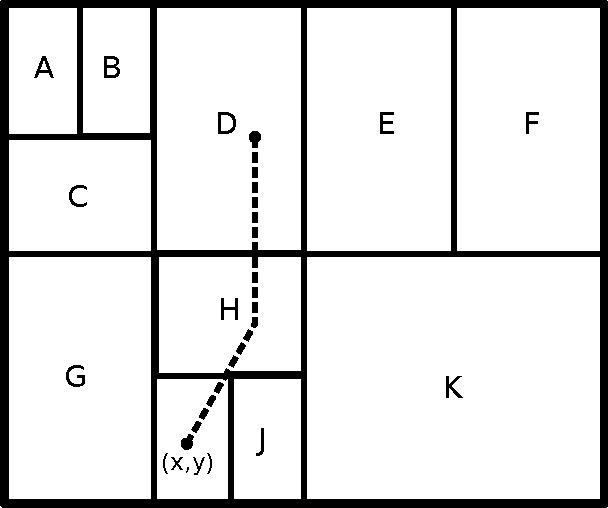
\includegraphics[scale=0.4]{img/algorithms/landmark_binning}
% \caption{Example 2D coordinate overlay and a sample routing path from node D to
% (x,y).}
% \label{fig:landmark_binning}
% \end{figure*}

\emph{Landmark Binning}~\cite{RHKS2002} partitions close-by nodes
into bins based on their distance from well known anchor nodes across the
Internet.%, as shown in Figure~\ref{fig:landmark_binning}.
To detect locality, peers mainly use network latency (i.e., \emph{RTT}).
%  as a measurement technique. 
Despite the fact that such delays are not always accurate,
they are used in~\cite{RHKS2002} for they are
non-intrusive, transparent and easy to apply.
%%
For the binning to work, a few anchor servers with known
physical locations need to be installed in strategic positions 
across the Internet. 
It is conjectured~\cite{RHKS2002} that $12$ such servers can prove
sufficient for the task.
An arriving node measures its distance from these landmarks
and unilaterally decides to join a specific bin based on its measurements.
%
%%VM Rewrote the following. Please double check that it makes sense. 
%%
Specifically, the node measures its round-trip time to each of the landmarks and
orders the landmarks in decreasing order of those \emph{RTT}-values.
Each permutation of the set of landmarks represents a specific bin. 
Should there $m$ landmarks be adopted, $m!$  different bins potentially exist. 
Peers that end up with the same ordering, belong to the same bin, in the sense that
if they experience similar overall latencies from fixed network points; it
is also  very likely that the peers in question are close to each other.
%%

As the operation of the method is independent of the model 
incorporated by the overlay network, the approach can be
applied with no significant changes to either
structured or unstructured \p\ systems.
%%
The rather obvious disadvantage of the approach lies in the
landmark servers that must be installed and maintained throughout the Internet.
Provided that a \p-system often may have a few million nodes 
connected at any given point in time, landmark servers do 
inherently play a pivotal role in the operation of the network. 
The approach has received a fair amount of criticism.
For instance, \cite{GSG2002} points out that end-hosts may bear the
cost of latency measurements and so, they may become bottlenecks.
\cite{CDCR2002,M2003,ZZZSZ2004}~argue that uneven distribution of nodes 
ultimately lead to load imbalances and \cite{RGJZ2004} indicates 
that its coarse-grained nature fails to
effectively distinguish among relatively close nodes.
Finally, \cite{XTZ2003} underscores the potentially increased maintenance cost(s).
%%%%%%%%%%%%%%%%%%%%%%%%%%%%%%%%%%%%%%
%%
%%
%
% Although latency estimation does not drain network resources,
% the scale of the approach does call for an alternative design.
% In this respect, \cite{RHKS2002} advocates the replacement of
% each landmark server by a cluster of servers.
% However, this approach may not entirely avoid the creation of 
% excessive network traffic flow through its landmark server-clusters.
%%
%%%%%%%%%%%%%%%%%%%%%%%%%%%%%%%%%%%%%%%%%%%%
%
%%
%To answer the question as to whether the algorithm actually contributes
% positively to the construction of an enhanced overlay, the paper defines the
%\emph{gain ratio} as the factor by which the latency reduces when someone
%communicates with a random node from the same bin than with one not in the bin.
%This is implemented with an inter-bin to an intra-bin latency ratio.
%
% TODO: LANDMARK BINNING FOR UNSTRUCTURED OVERLAYS
%
%For unstructured overlays the paper assumes \emph{a set of $n$ nodes where each
% node picks any $k$ neighbor nodes so that the average routing latency on the
%resultant overlay is low (assuming shortest path routing)}. According to the
%proposed heuristic algorithm called \emph{BinShort-Long}, a node picks its
%neighbors by choosing its $\frac{k}{2}$ closest\footnote{If the node's bin is
%not large enough for it to pick these $\frac{k}{2}$ neighbors, it picks the
%required nodes from the bin that matches the most in terms of landmark
%ordering.} ones (named \emph{short links}), using the \emph{binning} scheme and
%the rest $\frac{k}{2}$ randomly (\emph{long links}). The former set produces
%well-connected \emph{pockets} of nearby nodes while the later preserves the
%connectivity of the graph, both yielding a proximity factor of $\alpha = 0.5$
%in an attempt to preserve the beneficial properties of unstructured
%topologies\cite{merugu_str2unstr_2003}.
%
% TODO: SOME DISCUSSION
%
%A potential bottleneck could be the extra load that this
%``ping''-like scheme imposes to the landmarks, especially when we need instant
%reaction from our topology when dealing with the dynamic nature of the p2p
%networks.
%
%One disadvantage of this landmark scheme is related to the additional burden
% imposed to the landmark sites. The authors claim though that the algorithm
%requires so little work by the landmarks (maybe just echo to ping messages)
%that could in effect, act as ``unsuspecting participants''. Even if this is the
%case, the fact that it is not fully distributed, renders the protocol's
%scalability directly vulnerable to any system size increase as well as
%suitable for highly dynamic networks such as ad-hoc networks. Moreover, fixed
%points in a network are inherently more exposed to malicious attacks. The most
%significant downside of the algorithm though is that it can lead to an
%extremely uneven overlay ID distribution causing load unbalances and hot spots.
%Lastly, the scheme is coarse grained when it comes to distinguishing relatively
%close nodes\footnote{In the worst case, all nodes could ve clustered into a
%single bin.}.
%
%%
The landmark binning behaves as follows:
\begin{center}
{\footnotesize
\begin{tabular}{ccc}
\emph{Efficiency} & \emph{Overhead} & \emph{Scalability} \\
\hline
% The technique is coarse grained thus doesn't achieve optimal results
% (especially in small networks)
medium &
% The algorithm needs only nodes to compute distances to a small number of
% predefined nodes without exchanging any additional information.
low &
% The introduction of landmark servers renders the approach not fully
% decentralized, thus preventing it from scaling smoothly. Communicating
% and overloading landmark servers in high-churn systems is another scalability
% concern.
low
\end{tabular}
}
\end{center}

%%%%%%%%%%%%%%%%%%%%%%%%%%%%%%%%%%%%%%%%%%%%%%%%%%%%%%%%%%%%%%%%%%%%%%%%%%%%%%%%
% \subsubsection{mOverlay}
The \emph{mOverlay}~\cite{ZZZSZ2004} approach addresses scalability issues
that might arise when static landmark servers are in use.
To this end, the use of dynamic landmarks is proposed.
\emph{mOverlay}'s founding notion is that of a \emph{group} that 
designates a set of peers found in close proximity.
This proximity is user-defined in the protocol and 
may involve metrics including \emph{RTT}s and network latencies.
By and large a clustering approach, \emph{mOverlay} seeks to 
recreate small-world-like properties by producing a 
two-level hierarchical structure:
at the top level, there are only connections among groups 
while at the bottom, only \emph{intra-group} connections occur among peers.
%% 

Clearly, identifying groups and accurately finding the closest group 
to a peer is a fundamental concern in the creation of the overlay.
Nodes are grouped based on their distance to 
the groups already in the network, rendering
the latter be the \emph{dynamic landmarks} in the process. 
%%
For an incoming peer $Q$, 
the \emph{grouping criterion} designates that when the distance of $Q$ and
some group $A$'s neighbor groups is the same as the distance
between group $A$ and group $A$'s neighbor groups, then host $Q$
should belong to group $A$. 
During network initialization or when the grouping
criterion is not met, new groups are created.
A peer may reach its group by expending at most $O(logN)$ messages.
Finally, \emph{mOverlay} maintains stability and constant 
overheads when a host either fails or departs the network;
this is achieved through periodic cache updates and group 
leader selections, should a node either leaves or dies.
%
%\paragraph{Locating process} A new coming host, $Q$, first connects to a
%globally known host cache called the \emph{rendezvous point (RP)} in order to
%retrieve the starting point in the overlay, say $A$ in group $1$. Host $Q$
%then, measures its distance to host $A$. At the same time, the later, sends
%information about the neighbor groups of group $1$ back to host $Q$. This list
%is called \emph{candidate group list}, and the new coming host sequentially
%measures its distance to each of them in seek for the closest one. If the
%\emph{grouping criterion} is met, host $Q$ belongs to group $1$. If not, a boot
%host from the closest group is found and the algorithm is re-run until the
%criterion is met or after a predefined number of repetitions. In the later
%case, $Q$ creates a new group comprising itself only. The above protocol does
%not favor hot-spots as it spreads the probability of visiting a group across
%the whole overlay and limits the overhead in the level of $O \left ( log N
%\right )$.
%
%\paragraph{General overlay operations} A set of additional protocols, are also
% introduced, similar to those found in traditional unstructured networks, but
%modified focusing on scalability and robustness. For example a protocol for
%\emph{group formation} is introduced that exploits the inherent characteristic
%of proximity, in the overlay, in order to efficiently detect the neighboring
%groups of a newly formed group from the set of adjacent groups of its closest
%neighbor. Additionally, during \emph{group joining} the corresponding protocol
%denotes the exchange of important information for group maintenance. This can
%be further improved by \emph{information sharing} between nodes of the same
%group, functionality handled by a dedicated flood-like protocol\footnote{Since
%nodes that belong to the same group are physically close this can be achieved
%at a minimum price.}. Moreover, another set of distributed protocols handle the
%\emph{information update}. The information that needs update, in the proposed
%architecture, is
%\begin{inparaenum}[\itshape i\upshape)]
%  \item the host cache, when a new node joins, and
%  \item the neighbors of groups, when a close-by group is generated.
%\end{inparaenum}
%Finally, in case of \emph{host failure} or \emph{host departure} the system is
% able to maintain its stability since there are defined operations for
%periodical host cache update and group leader selection if one leaves or dies.
%
%%
In terms of the stated three criteria, \emph{mOverlay} fares as follows:
\begin{center}
{\footnotesize
\begin{tabular}{ccc}
\emph{Efficiency} & \emph{Overhead} & \emph{Scalability} \\
\hline
% The technique is coarse grained thus doesn't achieve optimal results
% (especially in small networks)
medium &
% The algorithm is iterative through the available groups. At each group
% probing of a candidate list must be performed. This process is done at
% bootstrapping time so the overhead increases in high-churn systems
medium &
% The introduction of dynamic landmark servers renders this approach much more
% scalable than the traditional static landmarking techniques 
medium
\end{tabular}
}
\end{center}

%%%%%%%%%%%%%%%%%%%%%%%%%%%%%%%%%%%%%%%%%%%%%%%%%%%%%%%%%%%%%%%%%%%%%%%%%%%%%%%%
%%%%%%%%%%%%%%%%%%%%%%%%%%%%%%%%%%%%%%%%%%%%%%%%%%%%%%%%%%%%%%%%%%%%%%%%%%%%%%%%
\subsection{Discussion on the Algorithms for Unstructured Architectures}
%%%%%%%%%%%%%%%%%%%%%%%%%%%%%%%%%%%%%%%%%%%%%%%%%%%%%%%%%%%%%%%%%%%%%%%%%%%%%%%%
%%%%%%%%%%%%%%%%%%%%%%%%%%%%%%%%%%%%%%%%%%%%%%%%%%%%%%%%%%%%%%%%%%%%%%%%%%%%%%%%




%%%%%%%%%%%%%%%%%%%%%%%%%%%%%%%%%%%%%%%%%%%%%%%%%%%%%%%%%%%%%%%%%%%%%%%%%%%%%%%%
%
% TODO: HOW CAN UNSTRUCTURED SCHEMES BE REFINED
%
%For this reasons, efforts have been placed for optimizing the efficiency of
%decentralized unstructured peer-to-peer networks. Research mainly focuses on
%\begin{inparaenum}[\itshape i\upshape)]
%  \item reducing unnecessary, redundant communication traffic, and
%  \item exploiting physical locality to reduce communication response.
%\end{inparaenum}
%The goal can be achieved at, both, the application-level network as well as the
%underlying physical one. In the first case by refining the message relay
%techniques, while in the second one, by adaptively reconstructing the
%application network to map as well as possible to the the physical network.
%
%%%%%%%%%%%%%%%%%%%%%%%%%%%%%%%%%%%%%%%%%%%%%%%%%%%%%%%%%%%%%%%%%%%%%%%%%%%%%%%%

While surveying efforts to overcome the mismatch problem
in the area of unstructured \p\ systems,
we came to identify four key methodologies 
utilized by the discussed approaches; they are:
\begin{enumerate}[\itshape i\upshape)]
  \item topology adaptation
  \item forwarding optimization
  \item caching and replication, and
  \item landmarking.
\end{enumerate}
%
A key characteristic shared by many of the presented techniques 
is that they do not strictly adhere to a single methodology.
As approaches attempt to address the challenging problem 
of topology mismatch, they resort to heuristics and so, 
they do not often furnish ``pure'' approaches that exclusively
belong to one of the $4$ aforementioned methodologies.
For instance, \emph{mOverlay} combines topology adaptation 
with landmark binning 
while \emph{Gia} weaves together $3$ methodologies:  topology adaptation, 
forwarding optimization and caching. 
This combination inevitably leads to feature/performance trade-offs: for example, 
the effectiveness of a caching/replication component can be undermined
by a continuously adapting overlay that removes important links between peers.
If a technique is to be evaluated for a specific application domain,
its overall approach as well as its underlying used methodologies have to be considered.
%%%%%%%%%%%%%%%%%%%%%%%%%%%%%%%%%%

In what follows, we outline how the surveyed protocols 
use elements of the above four methodologies. 
We then  offer a summary qualitative comparison for all surveyed
approaches applicable for \emph{unstructured}~\p~\emph{systems}.
Specifically, Table~\ref{unstructured:table} summarizes, for each
effort, the methodologies it incorporates, its special highlights as well as 
a rough estimation of the pros and cons in its implementation. 
Last but not least, Figures~\ref{unstructured:plot:efficiency}, \ref{unstructured:plot:overhead}
and \ref{unstructured:plot:scalability} pictorially compare the
surveyed techniques in terms of \emph{efficiency}, \emph{overhead} and \emph{scalability};
we defined these three criteria in Subsection~\ref{background:motivation}
and we collectively used them as a yardstick to qualitatively 
evaluate the presented approaches.

%%%%%%%%%%%%%%%%%%%%%%%%%%%%%%%%%%%%%%%%%%%%%%%%%%%%%%%%%%%%%%%%%%%%%%%%%%%%%%%%
\subsubsection{Topology Adaptation Methodology}

Protocols based on topology adaptation 
modify the topology of the \p\ network
using various schemes, the two most common of which
create either \emph{spanning tree}s using connection graphs
or \emph{clusters} of physically close nodes.

\emph{Narada} and subsequent algorithms including 
\emph{AOTO, LTM, SBO} try to solve the problem
by building ``a richer connected graph'' and by forming 
minimum spanning trees over
this graph that can efficiently route messages among peers. 
\emph{AOTO, LTM} and \emph{SBO} try to
overcome this limitation with ingenious schemes
like forming minimum spanning trees
for the $2$-hop away neighbors for each node, separating participant nodes into
groups, sometimes with different responsibilities and tasks at hand (e.g.,
\emph{SBO}). 
The advantage of building minimum spanning trees is that
they maintain the connectivity on the network in
an efficient manner while still preserving the overall search scope.
However, their construction and their update costs,
especially in dynamic and high-churn environments,
may cause large traffic overheads on the underlying
network~\cite{CRZ2000,CRSZ2001,CRSZ2002}.

The cluster-based approaches, on the other hand, 
link physically-close nodes to each other. 
\emph{T2MC}, for example, uses trace-route logs and 
\emph{DDNO} exploits domain names to cluster nodes in proximity at peer join.
Further enhancements may include dynamic local restructuring of the overlay
graph through neighbor exchange like in \emph{PROP} or cycle-cut like in
\emph{DCMP} to achieve continuous adaptation throughout a peer's life-cycle.
Unfortunately, commonly used methods for proximity detection across Internet do
not always return
reliable results and therefore, mapping accuracy is not guaranteed. Specifically
for traceroute, its overhead is not negligible and routers or firewalls in a
network may have already been configured to disable traceroute response from
the start. 
The most problematic aspect of clustering, though, is
its nature per se. 
Limited connectivity among the various local domains can
significantly shrink the search scope, negatively affecting the query response
time that the \p\ user experiences. 
%%
Among others, \emph{DDNO} tries to 
balance the efficiency of the clustering approach 
with enhanced node connectivity by forcing half of each node's connections to be
with other, randomly selected, nodes.

As a methodology, topology adaptation, ultimately aims to reduce the 
average path traversing cost from one node to another.
In doing so, the methodology re-arranges the
overlay network so that it becomes a better fit 
for the underlying \emph{IP} network
as Figure~\ref{figure:topology-adaptation} depicts.
Despite the fact that the above is a plausible proposition,
it is not always advantageous though. For example, a topology adaptive
algorithm can exchange a slow edge in the overlay with a faster one
thus reducing the average latency of the network communication.
The pitfall here is that this new virtual link
can traverse a fast \emph{AS}--to--\emph{AS} link meaning that even though
message round-trip-time is reduced, it has actually additional cost in terms of
inter-\emph{ISP} communication accounting and management.
%%
\begin{figure}[ht]
\centering
\subfigure[Inefficient overlay topology averaging $\simeq 16$ delay units.] {
  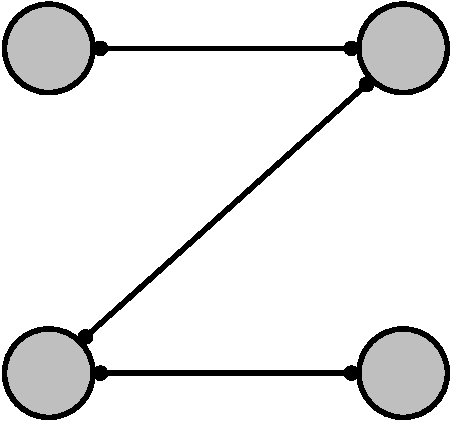
\includegraphics[scale=0.36]{img/pdf/topology-adaptation-before.pdf}
  \label{figure:topology-adaptation:before}
}\qquad\qquad
\subfigure[Efficient overlay topology after adaptation averaging $\simeq 11$ delay units.] {
  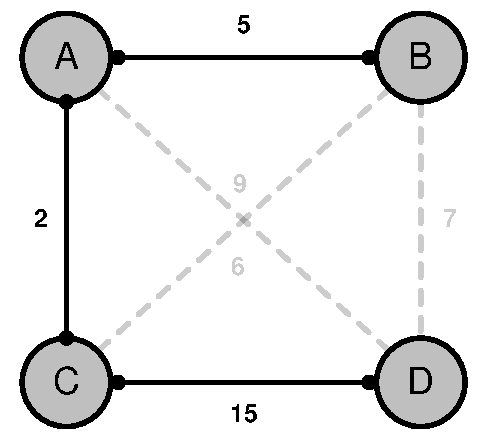
\includegraphics[scale=0.36]{img/pdf/topology-adaptation-after.pdf}
  \label{figure:topology-adaptation:after}
}
\caption{A simplified example on how overlay topology adaptation may improve matters.}
\label{figure:topology-adaptation}
\end{figure}
%%

%%%%%%%%%%%%%%%%%%%%%%%%%%%%%%%%%%%%%%%%%%%%%%%%%%%%%%%%%%%%%%%%%%%%%%%%%%%%%%%%
\subsubsection{Forwarding Optimization Methodology}
In unstructured systems, there is no way to know where data are actually located. 
This is why early works like Gnutella \cite{gnutellav04} used blind flooding, 
a \emph{BFS}--approach with depth $d$ and a system-maximum \emph{TTL} value 
(in terms of hops) for messages. 
This is inefficient since it generates a large number of
messages, a lot of which are duplicates. 
Approaches based on \emph{forwarding-optimization} propose 
intelligent search mechanisms in an attempt to
make searching more efficient.

Figure~\ref{figure:forwarding-optimisation} shows a simple example
of how forwarding optimization may work.
%%
\begin{figure}[ht]
\centering
\subfigure[Typical blind flooding.] {
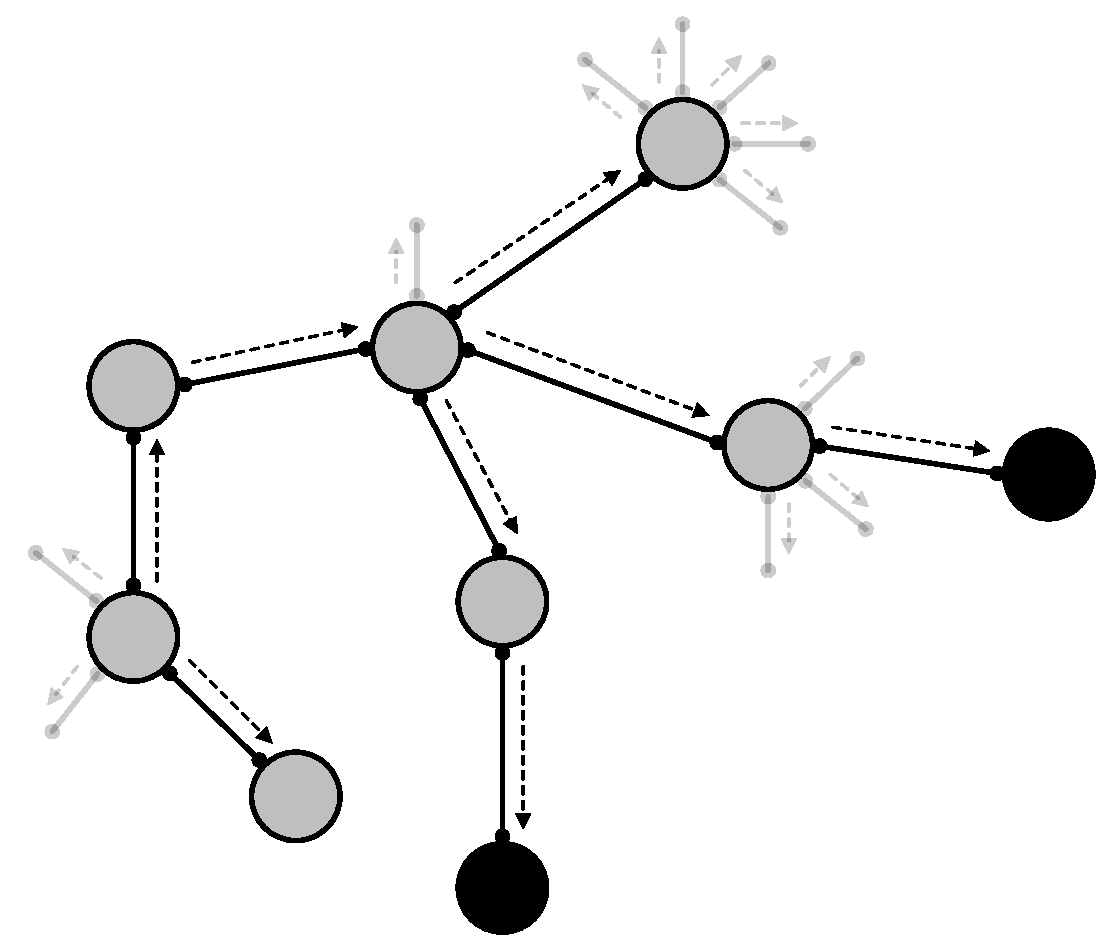
\includegraphics[scale=0.17]{img/pdf/forwarding-optimization-before.pdf}
  \label{figure:forwarding-optimisation:before}
}\qquad\qquad
\subfigure[A node can decide where to forward the messages.] {
  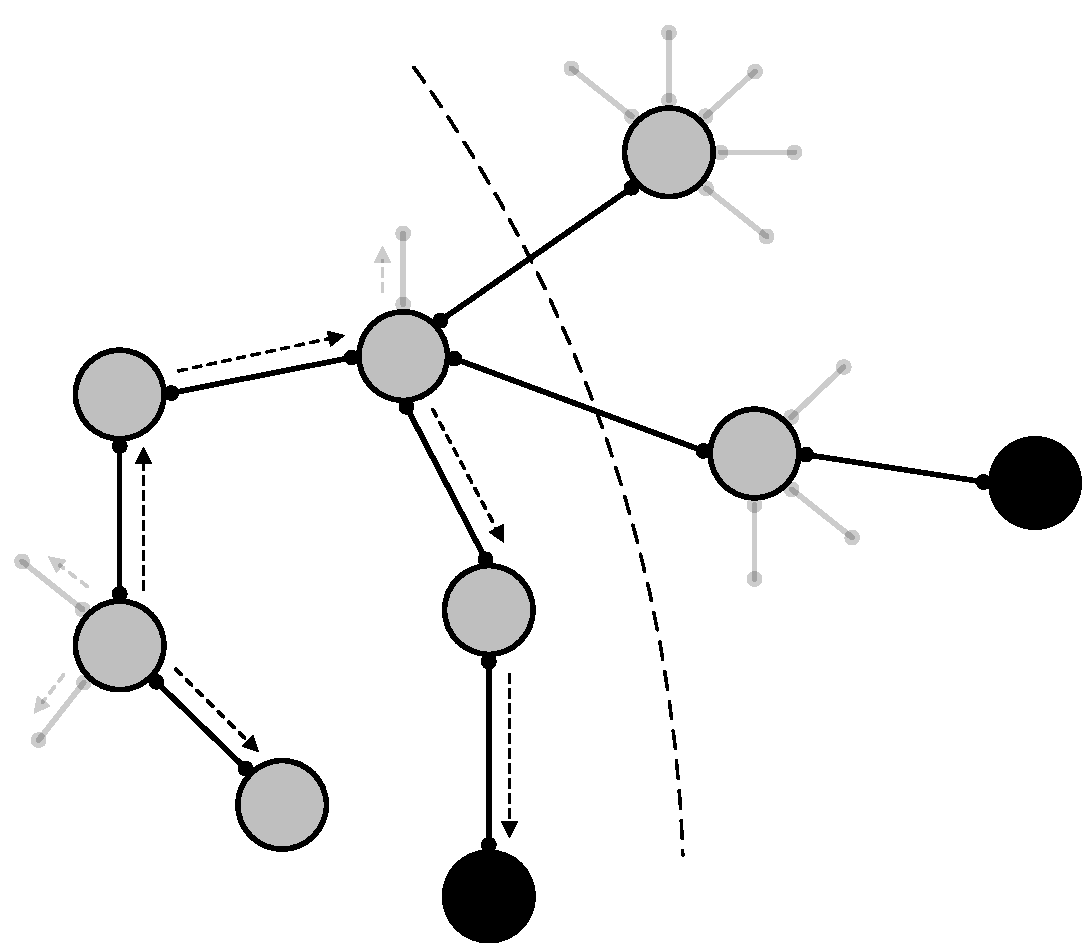
\includegraphics[scale=0.19]{img/pdf/forwarding-optimization-after.pdf}
  \label{figure:forwarding-optimisation:after}
}
\caption{Forwarding optimization in constraining message flooding.}
\label{figure:forwarding-optimisation}
\end{figure}
%%
Fig.~\ref{figure:forwarding-optimisation:before} 
shows a protocol that simply floods the entire network 
in search of object found in the nodes colored in black.
Alternatively, a node can decide to forward its
messages not to every output link but to a specific 
or subset of its outgoing links.
In Fig.~\ref{figure:forwarding-optimisation:after}, 
the node in the middle, does not flood its neighbors as instead 
it only picks one of them.
The dashed line on the right, shows that, 
for this routing process, the protocol has
rendered two potential forwarding paths as inefficient (e.g., the target nodes
show overloading signs).

Many alternative schemes have been proposed for this category, some of which we
have surveyed; iterative deepening, modified \emph{BFS}, local indices \cite{YG-M2002},
$k$-walker random walks \cite{LCCLS2002} or heterogeneity exploitation and
token-based flow control mechanisms \cite{CRBLS2003}. More sophisticated
alternatives also exist, taking into account application--level requirements
or even exploiting machine learning techniques to adjust overlay network
routing \cite{BFLZ2003}.

Forwarding-optimization schemes in unstructured \p\ systems can be classified
as \emph{DFS-} or \emph{BFS}-based. Routing indices \cite{CG-M2002} for example is a
\emph{DFS}-based technique while all the aforementioned are \emph{BFS}. Also,
the schemes in question can
be classified as deterministic or probabilistic (probabilistic, random or
ranking-based query forwarding). Iterative deepening and local indices
\cite{YG-M2002} are examples of deterministic approaches. Moreover, in the
literature algorithms are also taxonomised as blind or informed depending on
whether nodes keep some metadata to facilitate the search. For example,
$k$-walker random walks or iterative deepening are considered blind searches
while local indices informed.

On one hand, forward-optimization approaches have 
the advantage of enhancing the
search responsiveness and reducing the aggregate resource 
usage of the physical network. On the other, 
they suffer from drastic reduction of the search
scope (in Fig.~\ref{figure:forwarding-optimisation:after} the object on
the far right is not reached) thus, limiting the scalability of the whole
network. 
Forward-optimization suggestions address the problem of the mismatch 
in a limited manner since they do not provide any guarantees 
that overlay and underlying topologies are
aligned with each other.
To this end, forward-optimization techniques are commonly applied in
conjunction with other methodologies to improve 
the overall quality of \p\ systems.


%%%%%%%%%%%%%%%%%%%%%%%%%%%%%%%%%%%%%%%%%%%%%%%%%%%%%%%%%%%%%%%%%%%%%%%%%%%%%%%%
\subsubsection{Caching and Replication Methodology}

Caching is widely used to exploit locality and minimize redundant
transfer of data. Caching has with much success been successfully 
adopted by web-- and file--server application environments. 
Since peers in a \p\ system also operate as servers,
it is intuitively expected that \p\ file--sharing systems can also benefit from
caching in improving performance and reducing overall resource usage. 
However, the design of caches in this context 
is non-trivial compared to the web-based caching. 
Due to the fact nodes play the double role of server and client,
two important issues have to be considered at design time. 
First, the lifetime of a query is short, as the nodes join 
and leave frequently. Second, the result
of a single query string is not always the same, as this depends on the
source of the query, the \emph{TTL} value set for the messages, 
the current interconnection of peers and the 
high volatility of the environment. 
Thus, to develop a successful caching system for a \p\ architecture, these
parameters also have to be carefully considered. 
\p\ caching/replication can be applied
at two different levels, namely caching indices or pointers to data 
(Fig.~\ref{figure:replication:index}) or caching the data itself 
(Fig.~\ref{figure:replication:data}). 
%%%
\begin{figure}[ht]
\centering
\subfigure[Indexing can reduce the cost of the last hop.] {
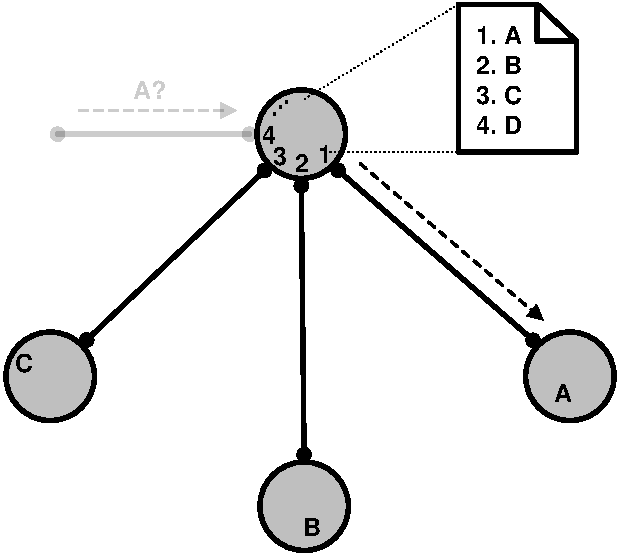
\includegraphics[scale=0.25]{img/pdf/replication-index.pdf}
  \label{figure:replication:index}
}\qquad\qquad
\subfigure[Data replication along the path of a successful query.] {
  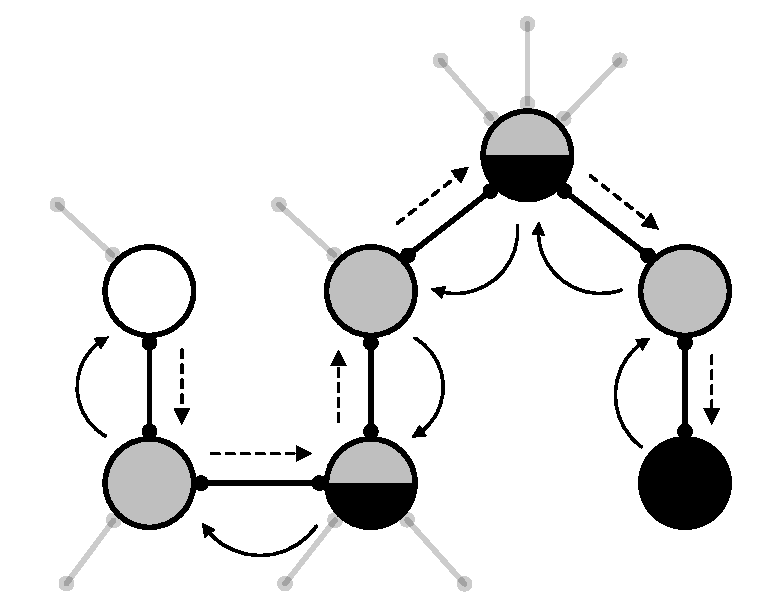
\includegraphics[scale=0.25]{img/pdf/replication-data.pdf}
  \label{figure:replication:data}
}
\caption{Index and data replication strategies.}
\label{figure:replication}
\end{figure}
%%
Successful implementations have
already been developed in some commercial \p\ systems, like 
\emph{KaZaA} or less popular ones including \emph{Gia} and \emph{BNS}.
%%%
Even though the state of the art in \p\ protocols using caching methods
helps reduce the burden of network resources, 
their contribution in addressing the actual mismatch between the overlay
and the underlying networks remains limited.

% TODO SOME DISCUSSION
%The caching policy varies depending on the way protocol handles the
%index and the
%content. Centralized P2P systems
%use central index servers, while local caching systems, such as KazaA, use
%super peers
%to cache indices in a distributed way. Content caching is also possible in P2P
%systems, where nodes cache the forwarded content for further retrievals.
%Although caching has the above mentioned advantages,  duplication
%of messages still exist, which limits the scalability of these approaches.
%Therefore, cache based approaches are analyzed in the following categories:
%  \begin{itemize}
%    \item \emph{data index caching},
%    \item \emph{content index caching},
%    \item \emph{centralized}, and
%    \item \emph{local}.
%  \end{itemize}

%%%%%%%%%%%%%%%%%%%%%%%%%%%%%%%%%%%%%%%%%%%%%%%%%%%%%%%%%%%%%%%%%%%%%%%%%%%%%%%%
\subsubsection{Landmarking}\label{sec:landmark}

In landmark-based algorithms, nodes use network delay (e.g., \emph{RTT}) as a
distance measurement method to position themselves with respect to ``a priori''
known servers on the Internet, like \emph{Ono} which uses the \emph{CDN}-infrastructure
for this purpose.

\begin{figure}[ht]
\centering
  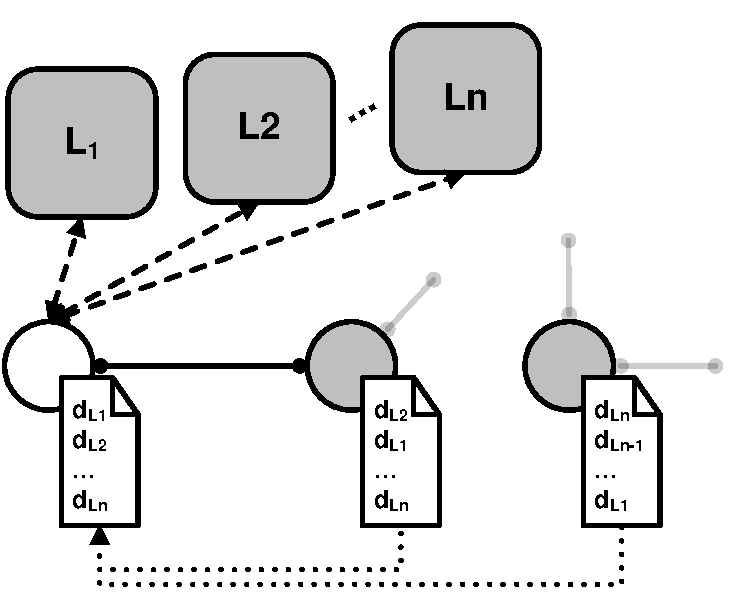
\includegraphics[scale=0.34]{img/pdf/landmarking.pdf}
\caption{Landmark binning during node bootstrap.}
\label{figure:landmarking}
\end{figure}

%\renewcommand\arraystretch{1.9}% (MyValue=1.0 is for standard)

\begin{landscape}
%\begin{figure}[h!]
\hspace{-3ex}
\begin{center}
\footnotesize
%\begin{tabular}{
\begin{longtable}{
|m{2cm}
|m{1cm}
|m{1cm}
|m{1cm}
|m{1cm}
|m{3cm}
|m{5cm}
|
}
% |>{\columncolor[gray]{.7}}m{0.1\columnwidth}
% |>{\columncolor[gray]{.9}}m{0.1\columnwidth}
% |>{\columncolor[gray]{.8}}m{0.1\columnwidth}
% |>{\columncolor[gray]{.9}}m{0.1\columnwidth}
% |>{\columncolor[gray]{.9}}m{0.1\columnwidth}
% |>{\columncolor[gray]{.8}}m{0.1\columnwidth}
% |>{\columncolor[gray]{.9}}m{0.1\columnwidth}
% |}
\caption[Summary table for unstructured algorithms]{Summary table for unstructured algorithms.} \label{unstructured:table} \\
\hline
%%%%%%%%%%%%%%%%%%%%%%%%%%%%%%%%%%%%%%%%%%%%%%%%%%%%%%%%%%%%%%%%%%%%%%%%%%%%%%%%
% first head
\rowcolor[gray]{.5}
\textbf{Algorithm / Paper} &
\textbf{Topology Adaptation} &
\textbf{Forwarding Optimization} &
\textbf{Caching / Replication} &
\textbf{Landmarking} &
\textbf{Highlights} &
\textbf{Pros / Cons}\\
\hline
\endfirsthead
%%%%%%%%%%%%%%%%%%%%%%%%%%%%%%%%%%%%%%%%%%%%%%%%%%%%%%%%%%%%%%%%%%%%%%%%%%%%%%%%
% subsequent heads
\multicolumn{7}{c}%
{\tablename\ \thetable\ -- \textit{Continued from previous page}} \\
\hline
\rowcolor[gray]{.5}
\textbf{Algorithm / Paper} &
\textbf{Topology Adaptation} &
\textbf{Forwarding Optimization} &
\textbf{Caching / Replication} &
\textbf{Landmarking} &
\textbf{Highlights} &
\textbf{Pros / Cons}\\
\hline
\endhead
%%%%%%%%%%%%%%%%%%%%%%%%%%%%%%%%%%%%%%%%%%%%%%%%%%%%%%%%%%%%%%%%%%%%%%%%%%%%%%%%
% foot
\hline \multicolumn{7}{r}{\textit{Continued on next page}} \\
\endfoot
%%%%%%%%%%%%%%%%%%%%%%%%%%%%%%%%%%%%%%%%%%%%%%%%%%%%%%%%%%%%%%%%%%%%%%%%%%%%%%%%
% last foot
\hline
\endlastfoot
%%%%%%%%%%%%%%%%%%%%%%%%%%%%%%%%%%%%%%%%%%%%%%%%%%%%%%%%%%%%%%%%%%%%%%%%%%%%%%%%
% data
\textbf{\cite{YG-M2002}} &
{\large \Square} &
{\large \CheckedBox} &
{\large \CheckedBox} &
{\large \Square} &
\begin{tabular}[l]{m{3cm}}
Iterative Deepening (ID).\\
Directed BFS (DBFS).\\
Local Indices (LI).
\end{tabular} &
\begin{tabular}[l]{m{5cm}}
+ ID reduces the messages especially in upper levels of the tree.\\
%+ DBFS ??????\\
+ LI reduces aggregate bandwidth usage and improves query efficiency.\\
-- ID needs evaluation time between iterations.\\
-- DBFS uses heuristics so it depends on their efficient choice.\\
-- LI add index update overhead which might be heavy process especially in high-churn systems.
\end{tabular}
\\
\hline
%%%%%%%%%%%%%%%%%%%%%%%%%%%%%%%%%%%%%%%%%%%%%%%%%%%%%%%%%%%%%%%%%%%%%%%%%%%%%%%%
\textbf{DAPS \cite{ZL2005}} &
{\large \Square} &
{\large \Square} &
{\large \Square} &
{\large \Square} &
\begin{tabular}[l]{m{3cm}}
Clustered routing tables based on delay.\\
Pruning flood, an iterative deepening and multiple BFS approach with a pruning
boundary.
\end{tabular} &
+ It is a system between structured and unstructured.
\\
\hline
%%%%%%%%%%%%%%%%%%%%%%%%%%%%%%%%%%%%%%%%%%%%%%%%%%%%%%%%%%%%%%%%%%%%%%%%%%%%%%%%
\textbf{Gia \cite{CRBLS2003}} &
{\large \CheckedBox} &
{\large \CheckedBox} &
{\large \CheckedBox} &
{\large \Square} &
\begin{tabular}{m{3cm}}
Random Walks (RW).
\end{tabular} &
\begin{tabular}[l]{m{5cm}}
+ RWs issue one copy of the query thus not flooding the whole network.\\
-- RWs can reduce search scope.\\
\end{tabular}
\\
\hline
%%%%%%%%%%%%%%%%%%%%%%%%%%%%%%%%%%%%%%%%%%%%%%%%%%%%%%%%%%%%%%%%%%%%%%%%%%%%%%%%
\textbf{DCMP \cite{ZKB2008}} &
{\large \CheckedBox} &
{\large \Square} &
{\large \Square} &
{\large \Square} &
\begin{tabular}{m{3cm}}
Cycle detection.
\end{tabular} &
\begin{tabular}[l]{m{5cm}}
+ Drastically reduces duplicate messages.\\
-- Cannot detect cycles in distance bigger than the TTL value of the IC message.\\
\end{tabular}
\\
\hline
%%%%%%%%%%%%%%%%%%%%%%%%%%%%%%%%%%%%%%%%%%%%%%%%%%%%%%%%%%%%%%%%%%%%%%%%%%%%%%%%
\textbf{\cite{CS2002}} &
{\large \Square} &
{\large \Square} &
{\large \CheckedBox} &
{\large \Square} &
\begin{tabular}[l]{m{3cm}}
Uniform replication.\\
Proportional replication.\\
Square root replication allocation.
\end{tabular} &
\begin{tabular}[l]{m{5cm}}
+ Uniform replication reduces time spend on unsuccessful searches.\\
+ Reduces search time for frequent queries.\\
-- Proportional replication struggles in locating rare objects.
\end{tabular}
\\
\hline
%%%%%%%%%%%%%%%%%%%%%%%%%%%%%%%%%%%%%%%%%%%%%%%%%%%%%%%%%%%%%%%%%%%%%%%%%%%%%%%%
% \textbf{Tracing a large-scale Peer to Peer System: an hour in the life of Gnutella} &
% ? &
% ? &
% ? &
% ? &
% ? &
% ?
% \\
% \hline
%%%%%%%%%%%%%%%%%%%%%%%%%%%%%%%%%%%%%%%%%%%%%%%%%%%%%%%%%%%%%%%%%%%%%%%%%%%%%%%%
\textbf{Narada \cite{CRZ2000}} &
{\large \Square} &
{\large \CheckedBox} &
{\large \Square} &
{\large \Square} &
\begin{tabular}[l]{m{3cm}}
Mess creation.\\
Minimum spanning trees.
\end{tabular} &
\begin{tabular}[l]{m{5cm}}
+ Mess and trees are kept up to date in high churn environments.\\
-- Works well only for small groups of peers.
\end{tabular}
\\
\hline
%%%%%%%%%%%%%%%%%%%%%%%%%%%%%%%%%%%%%%%%%%%%%%%%%%%%%%%%%%%%%%%%%%%%%%%%%%%%%%%%
\textbf{AOTO \cite{LZXN2003}} &
{\large \CheckedBox} &
{\large \CheckedBox} &
{\large \Square} &
{\large \Square} &
\begin{tabular}[l]{m{3cm}}
Minimum spanning trees.\\
Peer proximity heuristic for removing costly links.
\end{tabular} &
\begin{tabular}[l]{m{5cm}}
+ Spanning trees only to immediate neighbors so no flooding and at the same time
no shrinked search scope.\\
+ Selective flooding effectiveness is detached from physical or overlay topologies.\\
+ The more logical neighbors, the more effective selective flooding becomes\\
-- High recalculation costs.\\
-- No sophisticated selection policy for candidate non-flooding peers.
\end{tabular}
\\
\hline
%%%%%%%%%%%%%%%%%%%%%%%%%%%%%%%%%%%%%%%%%%%%%%%%%%%%%%%%%%%%%%%%%%%%%%%%%%%%%%%%
\textbf{ACE \cite{LZXN2004}} &
{\large \CheckedBox} &
{\large \CheckedBox} &
{\large \Square} &
{\large \Square} &
\begin{tabular}[l]{m{3cm}}
Minimum spanning trees.\\
1-hop proximity heuristic.
\end{tabular} &
\begin{tabular}[l]{m{5cm}}
+ No flooding.\\
+ Less overhead compared to AOTO since computation is done within a certain diameter from the source peer.
-- Slow convergence speed.\\
-- Enhanced topology optimization comes to the expence of higher communication/computation overhead.
\end{tabular}
\\
\hline
%%%%%%%%%%%%%%%%%%%%%%%%%%%%%%%%%%%%%%%%%%%%%%%%%%%%%%%%%%%%%%%%%%%%%%%%%%%%%%%%
\textbf{LTM \cite{LLXNZ2004}} &
{\large \CheckedBox} &
{\large \Square} &
{\large \Square} &
{\large \Square} &
\begin{tabular}[l]{m{3cm}}
TTL detector (2-hop distance).\\
Delayed low productive connection cutting.
\end{tabular} &
\begin{tabular}[l]{m{5cm}}
+ Compared to AOTO, ACE and SBO achieves faster convergence speed.\\
-- Creates more overhead than AOTO, ACE and SBO.\\
-- Needs synchronization of peer clocks.\\
-- Does not consider shortcuts created by powerful peers when choosing to disable connections (only uses delay metric).
\end{tabular}
\\
\hline
%%%%%%%%%%%%%%%%%%%%%%%%%%%%%%%%%%%%%%%%%%%%%%%%%%%%%%%%%%%%%%%%%%%%%%%%%%%%%%%%
\textbf{SBO \cite{LXN2004}} &
{\large \CheckedBox} &
{\large \CheckedBox} &
{\large \Square} &
{\large \Square} &
\begin{tabular}{m{3cm}}
Red/white bipartite overlay.
\end{tabular} &
\begin{tabular}[l]{m{5cm}}
+ Efficient in both static and dynamic environments.\\
+ Compared to AOTO incurs half the overhead.\\
-- Needs almost double the steps of LTM to converge (static or dynamic environments).
\end{tabular}
\\
\hline
%%%%%%%%%%%%%%%%%%%%%%%%%%%%%%%%%%%%%%%%%%%%%%%%%%%%%%%%%%%%%%%%%%%%%%%%%%%%%%%%
\textbf{THANCS \cite{LNXE2005}} &
{\large \CheckedBox} &
{\large \CheckedBox} &
{\large \Square} &
{\large \Square} &
\begin{tabular}[l]{m{3cm}}
Local optimum heuristic\\
Piggybacking neighbor distance in queries
\end{tabular} &
\begin{tabular}[l]{m{5cm}}
+ Completely distributed approach.\\
+ Presents trivial overhead compared to the query cost savings.\\
+ Convergent speed faster among AOTO, LTM, SBO.\\
+ Does not shrink the search scope.\\
-- Design cannot be extended to support non-flooding-based systems.
\end{tabular}
\\
\hline
%%%%%%%%%%%%%%%%%%%%%%%%%%%%%%%%%%%%%%%%%%%%%%%%%%%%%%%%%%%%%%%%%%%%%%%%%%%%%%%%
\textbf{HAND \cite{CLZHC2006}} &
{\large \CheckedBox} &
{\large \Square} &
{\large \Square} &
{\large \Square} &
\begin{tabular}{m{3cm}}
Triple-hop adjustment.
\end{tabular} &
\begin{tabular}[l]{m{5cm}}
+ No need for clock sync.\\
+ Fully distributed.\\
+ Low overhead for the triple hop adjustment.\\
+ Applicable to both static and dynamic environments.\\
+ Low query response time.\\
-- Compared to LTM has lower traffic reduction and query response rates.
\end{tabular}
\\
\hline
%%%%%%%%%%%%%%%%%%%%%%%%%%%%%%%%%%%%%%%%%%%%%%%%%%%%%%%%%%%%%%%%%%%%%%%%%%%%%%%%
\textbf{APS \cite{BFLZ2003}} &
{\large \CheckedBox} &
{\large \Square} &
{\large \Square} &
{\large \Square} &
\begin{tabular}{m{3cm}}
machine learning adaptive mechanism.
\end{tabular} &
\begin{tabular}[l]{m{5cm}}
+ Fully dynamic switching decision policy.\\
- Low convergence due to the learning process.
\end{tabular}
\\
\hline
%%%%%%%%%%%%%%%%%%%%%%%%%%%%%%%%%%%%%%%%%%%%%%%%%%%%%%%%%%%%%%%%%%%%%%%%%%%%%%%%
\textbf{ITA \cite{PRFM2009}} &
{\large \CheckedBox} &
{\large \CheckedBox} &
{\large \Square} &
{\large \Square} &
\begin{tabular}[l]{m{3cm}}
Short/long connections.\\
Local flooding.
\end{tabular} &
\begin{tabular}[l]{m{5cm}}
+ Low clustering.\\
+ Large peer coverage.\\
+ Reduced duplication.\\
+ Low or no impact to other mechanisms of unstructured p2p networks (e.g. 1-hop
replication, dynamic querying).
\end{tabular}
\\
\hline
%%%%%%%%%%%%%%%%%%%%%%%%%%%%%%%%%%%%%%%%%%%%%%%%%%%%%%%%%%%%%%%%%%%%%%%%%%%%%%%%
\textbf{EGOIST \cite{SLLBBR2008}} &
{\large \CheckedBox} &
{\large \Square} &
{\large \Square} &
{\large \Square} &
\begin{tabular}{m{3cm}}
Selfish shortest path routing
\end{tabular} &
\begin{tabular}{m{3cm}}
-- constructs a global view of the network
\end{tabular}
\\
\hline
%%%%%%%%%%%%%%%%%%%%%%%%%%%%%%%%%%%%%%%%%%%%%%%%%%%%%%%%%%%%%%%%%%%%%%%%%%%%%%%%
\textbf{BNS \cite{BCCMSBZ2006}} &
{\large \CheckedBox} &
{\large \Square} &
{\large \CheckedBox} &
{\large \Square} &
\begin{tabular}[l]{m{3cm}}
ISP clustering (tracker-side or ISP-side detection).\\
Bandwidth throttling.\\
Caching.
\end{tabular} &
\begin{tabular}[l]{m{5cm}}
+ Localizes traffic within an ISP.\\
+ Preserves the efficiency of BitTorrent protocol.\\
-- Needs ISPs to either provide information or infrastructure changes.\\
-- Locality-based approaches do not treat fair all peers.
\end{tabular}
\\
\hline
%%%%%%%%%%%%%%%%%%%%%%%%%%%%%%%%%%%%%%%%%%%%%%%%%%%%%%%%%%%%%%%%%%%%%%%%%%%%%%%%
\textbf{Ono \cite{CB2008}} &
{\large \CheckedBox} &
{\large \Square} &
{\large \Square} &
{\large \CheckedBox} &
\begin{tabular}[l]{m{3cm}}
ISP clustering.\\
Landmarking based on existing CDN infrastructure (CDN redirection measurements).
\end{tabular} &
\begin{tabular}[l]{m{5cm}}
+ Needs no ISP cooperation.\\
+ Needs no extra infrastructure.\\
+ Needs no network topology information.\\
-- Locality based approaches do not treat fair all peers.
\end{tabular}
\\
\hline
%%%%%%%%%%%%%%%%%%%%%%%%%%%%%%%%%%%%%%%%%%%%%%%%%%%%%%%%%%%%%%%%%%%%%%%%%%%%%%%%
\textbf{\cite{LCLX2009}} &
{\large \CheckedBox} &
{\large \Square} &
{\large \Square} &
{\large \Square} &
\begin{tabular}{m{3cm}}
AS hop count minimization on neighbor selection, on chocking/unchocking
mechanisms and on next-chunk picking.
\end{tabular} &
\begin{tabular}[l]{m{5cm}}
+ Optimization of the inter-AS traffic.\\
-- Locality based approaches do not treat fair all peers.
\end{tabular}
\\
\hline
%%%%%%%%%%%%%%%%%%%%%%%%%%%%%%%%%%%%%%%%%%%%%%%%%%%%%%%%%%%%%%%%%%%%%%%%%%%%%%%%
\textbf{TopBT \cite{RTLCGZ2010}} &
{\large \CheckedBox} &
{\large \Square} &
{\large \Square} &
{\large \Square} &
\begin{tabular}[l]{m{3cm}}
Peer selection metric that takes both downloading speed and network topology
into account.\\
Applied in multiple places of the BitTorrent protocol (bootstrap, connection
establishment/replacement, unchocking).
\end{tabular} &
\begin{tabular}[l]{m{5cm}}
+ No need for additional infrastructure.\\
+ Enhances both traffic and downloading.\\
-- Needs off-line processing of BGP dumps.
\end{tabular}
\\
\hline
%%%%%%%%%%%%%%%%%%%%%%%%%%%%%%%%%%%%%%%%%%%%%%%%%%%%%%%%%%%%%%%%%%%%%%%%%%%%%%%%
\textbf{UTAPS \cite{LCY2008}} &
{\large \CheckedBox} &
{\large \Square} &
{\large \Square} &
{\large \CheckedBox} &
\begin{tabular}{m{3cm}}
Network tomography to construct a picture for the underlying network.
\end{tabular} &
\begin{tabular}[l]{m{5cm}}
+ Reduced ISP burden.\\
+ Better downloading speeds.\\
-- Small, laboratory-scale evaluation setup.
\end{tabular}
\\
\hline
%%%%%%%%%%%%%%%%%%%%%%%%%%%%%%%%%%%%%%%%%%%%%%%%%%%%%%%%%%%%%%%%%%%%%%%%%%%%%%%%
\textbf{\cite{QLZG2009}} &
{\large \CheckedBox} &
{\large \Square} &
{\large \Square} &
{\large \CheckedBox} &
\begin{tabular}{m{3cm}}
Cluster peers in a swarm into local, intra- and inter-ISP.
\end{tabular} &
\begin{tabular}[l]{m{5cm}}
+ Reduced ISP burden.\\
+ Better downloading speeds.\\
-- Similarly to UTAPS, the evaluation setup was small scale.
\end{tabular}
\\
\hline
%%%%%%%%%%%%%%%%%%%%%%%%%%%%%%%%%%%%%%%%%%%%%%%%%%%%%%%%%%%%%%%%%%%%%%%%%%%%%%%%
\textbf{PROP \cite{QCYCZ2007}} &
{\large \CheckedBox} &
{\large \Square} &
{\large \Square} &
{\large \Square} &
\begin{tabular}{m{3cm}}
Neighbor exchange between peers.
\end{tabular} &
\begin{tabular}[l]{m{5cm}}
+ Cooperation between peers.\\
+ Guarantees the connectivity of the network between exchanges.\\
\end{tabular}
\\
\hline
%%%%%%%%%%%%%%%%%%%%%%%%%%%%%%%%%%%%%%%%%%%%%%%%%%%%%%%%%%%%%%%%%%%%%%%%%%%%%%%%
% \textbf{Resolving the Topology Mismatch Problem in Unstructured Peer-to-Peer Networks} &
% ? &
% ? &
% ? &
% ? &
% ? &
% ?
% \\
% \hline
%%%%%%%%%%%%%%%%%%%%%%%%%%%%%%%%%%%%%%%%%%%%%%%%%%%%%%%%%%%%%%%%%%%%%%%%%%%%%%%%
\textbf{DDNO \cite{Z-YK2005}} &
{\large \CheckedBox} &
{\large \Square} &
{\large \Square} &
{\large \Square} &
\begin{tabular}{m{3cm}}
Domain name topology detection (Split-Hash and dnMatch).
\end{tabular} &
\begin{tabular}[l]{m{5cm}}
+ Can be applied to both fully unstructured and super-peer based architectures.\\
+ Secures connectivity of the network.\\
+ Reduces cost of message exchange.
\end{tabular}
\\
\hline
%%%%%%%%%%%%%%%%%%%%%%%%%%%%%%%%%%%%%%%%%%%%%%%%%%%%%%%%%%%%%%%%%%%%%%%%%%%%%%%%
\textbf{CTAG \cite{ZL2006}} &
{\large \CheckedBox} &
{\large \Square} &
{\large \Square} &
{\large \Square} &
\begin{tabular}{m{3cm}}
Clustering based on longest matching IP segment.
\end{tabular} &
\begin{tabular}{m{5cm}}
+ Focuses on both construction and adaptation.
\end{tabular}
\\
\hline
%%%%%%%%%%%%%%%%%%%%%%%%%%%%%%%%%%%%%%%%%%%%%%%%%%%%%%%%%%%%%%%%%%%%%%%%%%%%%%%%
\textbf{Landmark Binning \cite{RHMKS2002}} &
{\large \CheckedBox} &
{\large \Square} &
{\large \Square} &
{\large \CheckedBox} &
\begin{tabular}{m{3cm}}
Landmark binning.
\end{tabular} &
\begin{tabular}[l]{m{5cm}}
+ It is independent of the overlay model.\\
+ The technique can be considered scalable.\\
-- Uses not so reliable network latency metric (this can lead to load imbalance etc).\\
-- The use of landmark servers renders the technique not fully distributed.\\
-- Excessive traffic flow towards the landmark servers is possible.\\
-- Fixed points in a network are inherently more exposed to malicious attacks.\\
-- Coarse-grained scheme.
\end{tabular}
\\
\hline
%%%%%%%%%%%%%%%%%%%%%%%%%%%%%%%%%%%%%%%%%%%%%%%%%%%%%%%%%%%%%%%%%%%%%%%%%%%%%%%%
\textbf{mOverlay \cite{ZZZSZ2004}} &
{\large \CheckedBox} &
{\large \Square} &
{\large \Square} &
{\large \CheckedBox} &
\begin{tabular}{m{3cm}}
Dynamic landmarks.
\end{tabular} &
\begin{tabular}[l]{m{5cm}}
+ Fully distributed.\\
+ It is independent of the overlay model.\\
-- Coarse-grained scheme.
\end{tabular}
\\
\hline
%%%%%%%%%%%%%%%%%%%%%%%%%%%%%%%%%%%%%%%%%%%%%%%%%%%%%%%%%%%%%%%%%%%%%%%%%%%%%%%%


%\begin{tabular}[l]{@{}}
%+ ID reduces the messages especially in upper levels of the tree\\
%+ DBFS\\
%+ LI reduces aggregate bandwidth usage and improves query efficiency\\
%- ID needs evaluation time between iterations\\
%- DBFS uses heuristics so it depends on their efficient choice\\
%- LI add index update overhead which might be heavy and might not work at all in systems with high churn
%\end{tabular} &


%\textbf{Narada} & \textbf{Overlay optimization
%based}. Creates a mesh (richer connected graph) and builds minimum spanning
%trees on this mesh & & Small and sparse groups \\

%\hline
%\textbf{Gia} & \textbf{Broadcast based} Replaces
%Gnutella flooding with random walk, and introduces KaZaA style super-nodes.
%Uses
%dynamic topology adaptation protocol &
% Gnutella &  Better than Gnutella  \\

%\hline
%\textbf{Adaptive Overlay Topology Optimization} & \textbf{Overlay optimization
%based}. Creates overlay multi-cast tree with Selective Flooding protocol&
%Gnutella &  Better than Gnutella \\

% \hline
% \textbf{Location-aware Topology Matching} &
% \textbf{Overlay Optimization Based}. Uses \textit{TTL2-detector flooding}, \textit{low productive
% connection cutting}, and \textit{source peer probing}. & Gnutella &  Better than Gnutella \\
% 
% \hline
% \textbf{Replication Strategies in Unstructured P2P Networks} &
% \textbf{Cache Based}. Uses uniform, proportional and square root allocation
% strategies to replicate data. & Gnutella &  Better than Gnutella \\
% 
% % \hline
% \textbf{Tracing a large-scale Peer to Peer System: an hour in the life of Gnutella.} &
% \textbf{Cache Based}. Proposes a caching algorithm based on the traces of the Gnutella traffic & Gnutella & Better than Gnutella \\
% 
% \hline
% \textbf{Improving search in P2P networks} &
% \textbf{Broadcast Based}. Uses \textit{iterative deepening}, \textit{directed
% BFS}, and \textit{local indices} to improve efficiency. & Gnutella &  Better than Gnutella \\
% 
% \hline
% \textbf{Distributed Cycle Minimization Protocol} &
% \textbf{Broadcast based} Uses a decentralized cycle elimination protocol  &  &  \\
% 
% \hline
% \textbf{Scalable Bipartite Overlay} &
% \textbf{Overlay optimization based} Uses bipartite partition graph and builds
% local minimum spanning trees  & Gnutella  & Better than Gnutella \\
% 
% \hline
% \textbf{Adaptive Connection Establishment} &
% \textbf{Overlay optimization based} Forms Neighbor Cost Tables, builds local
% minimum spanning trees and perform local optimizations & Adaptive Overlay
% Topology Optimization (AOTO), Gnutella & Better than Gnutella \\

% \hline
% \textbf{Hops Adaptive Neighbor Discovery} &  & &  \\
% 
% \hline
% \textbf{Two-Hop-Away Neighbor Comparison and Selection (THANCS)} &
% \textbf{Overlay optimization based} Uses piggybacking to discover neighbor
% distances and selects neighbors  & Gnutella  & \\

% \hline
% \textbf{mOverlay} &\textbf{Landmark based proximity} Uses dynamic landmarks to find node locality
% & & Due to dynamic landmarks and grouping, more scalable than tree-based or mesh-based protocols \\
% 
% \hline
% \textbf{Distributed Domain Name Order (DDNO)} &
% \textbf{Overlay optimization based} Connects half of the nodes connections to
% the nodes in the same domain and the other half to random nodes, therefore
% supports locality and topological connection  &  & Yes, by using super
% peers \\

% \hline
% \textbf{Peer-exchange Routing Optimization Protocols} & \textbf{Overlay optimization based} Optimizes overlay by the exchange of
% neighbors among peers  & Can work with both decentralized structured and
% unstructured architecture & Yes \\

% \hline
% \textbf{MAY OMIT - I CHANGED IT TO STRUCTURED SINCE THERE IS A REFERENCE FOR
% DHT (OF COURSE IT MIGHT POSSIBLE TO BE APPLIED TO BOTH. MAYBE NEED TO CHECK) -
% T2MC} &
% \textbf{Overlay optimization based} Uses trace-route results for clustering
% the nodes  & & \\
% 
% \hline
% \textbf{Unnamed-unstructured} &
% \textbf{Overlay optimization based} Minimizes the communication delay and
% maximizes the broadcasting range & & Better than THANCS and mOverlay \\

% \hline
% \textbf{Landmark Binning} & \textbf{Landmark based proximity} Uses network latency to partition
% nodes into bins & Can work with both decentralized structured and unstructured architecture & \\
% 
% \hline
%\end{tabular}
\end{longtable}
\end{center}
\vspace{-2.5ex}
\vspace{-2.5ex}
%\end{figure}
\end{landscape}

%%%%%%%%%%%%%%%%%%%%%%%%%%%%%%%%%%%%%%%%%%%%%%%%%%%%%%%%%%%%%%%%%%%%%%%%%%%%%%%%
%%%%%%%%%%%%%%%%%%%%%%%%%%%%%%%%%%%%%%%%%%%%%%%%%%%%%%%%%%%%%%%%%%%%%%%%%%%%%%%%
%                             UNSTRUCTURED
%%%%%%%%%%%%%%%%%%%%%%%%%%%%%%%%%%%%%%%%%%%%%%%%%%%%%%%%%%%%%%%%%%%%%%%%%%%%%%%%
%%%%%%%%%%%%%%%%%%%%%%%%%%%%%%%%%%%%%%%%%%%%%%%%%%%%%%%%%%%%%%%%%%%%%%%%%%%%%%%%

%\pgfplotsset{width=7cm,compat=newest}

%%%%%%%%%%%%%%%%%%% EFFICIENCY %%%%%%%%%%%%%%%%%%%
\begin{landscape}
\begin{center}
\begin{tikzpicture}
\begin{axis}[
  xbar,
  bar width=7pt,
  xlabel=\emph{Efficiency},
  ylabel=\emph{Algorithm},
  symbolic x coords={low, medium, high},
  symbolic y coords={
    IterativeDeepening,
    DirectedBFS,
    LocalIndices,
    DAPS,
    Gia,
    DCMP,
    UniformReplication,
    ProportionalReplication,
    SqrtReplication,
    %Markatos02,
    Narada,
    AOTO,
    ACE,
    LTM,
    SBO,
    THANCS,
    HAND,
    APS,
    ITA,
    EGOIST,
    BNS,
    Ono,
    LiuEtAl,
    TopBT,
    UTAPS,
    QinEtAl,
    PROP-G,
    PROP-O,
    %hsiao_redblue_2009,
    DDNO,
    CTAG,
    LB,
    mOverlay
  },
  every axis y label/.style=
    {at={(ticklabel cs:0.5)},rotate=90,anchor=near ticklabel},
%   x tick label style={rotate=45,anchor=east},
  xtick=data, ytick=data,
%   ymin=low,ymax=high,ytickmin=low,
  height=\textheight - 0.3cm,
  width=\textwidth,
  enlargelimits=0.05,
  title=\emph{Efficiency} Pictorial Comparison of Unstructured Approaches.
]

\addplot[black,fill=gray!20, postaction={pattern=north east lines}]
table[x=EFFICIENCY,y=ALGORITHM]
{unstructured-plot.dat};

\end{axis}
\end{tikzpicture}
\end{center}
\end{landscape}

%%%%%%%%%%%%%%%%%%% OVERHEAD %%%%%%%%%%%%%%%%%%%
\begin{landscape}
\begin{center}
\begin{tikzpicture}
\begin{axis}[
  xbar,
  bar width=7pt,
  xlabel=\emph{Overhead},
  ylabel=\emph{Algorithm},
  symbolic x coords={low, medium, high},
  symbolic y coords={
    IterativeDeepening,
    DirectedBFS,
    LocalIndices,
    DAPS,
    Gia,
    DCMP,
    UniformReplication,
    ProportionalReplication,
    SqrtReplication,
    %Markatos02,
    Narada,
    AOTO,
    ACE,
    LTM,
    SBO,
    THANCS,
    HAND,
    APS,
    ITA,
    EGOIST,
    BNS,
    Ono,
    LiuEtAl,
    TopBT,
    UTAPS,
    QinEtAl,
    PROP-G,
    PROP-O,
    %hsiao_redblue_2009,
    DDNO,
    CTAG,
    LB,
    mOverlay
  },
  every axis y label/.style=
    {at={(ticklabel cs:0.5)},rotate=90,anchor=near ticklabel},
%   x tick label style={rotate=45,anchor=east},
  xtick=data, ytick=data,
%   ymin=low,ymax=high,ytickmin=low,
  height=\textheight - 0.3cm,
  width=\textwidth,
  enlargelimits=0.05,
  title=\emph{Overhead} Pictorial Comparison of Unstructured Approaches.
]

\addplot[black,fill=gray!20, postaction={pattern=crosshatch}]
table[x=OVERHEAD,y=ALGORITHM]
{unstructured-plot.dat};

\end{axis}
\end{tikzpicture}
\end{center}
\end{landscape}

%%%%%%%%%%%%%%%%%%% SCALABILITY %%%%%%%%%%%%%%%%%%%
\begin{landscape}
\begin{center}
\begin{tikzpicture}
\begin{axis}[
  xbar,
  bar width=7pt,
  xlabel=\emph{Scalability},
  ylabel=\emph{Algorithm},
  symbolic x coords={low, medium, high},
  symbolic y coords={
    IterativeDeepening,
    DirectedBFS,
    LocalIndices,
    DAPS,
    Gia,
    DCMP,
    UniformReplication,
    ProportionalReplication,
    SqrtReplication,
    %Markatos02,
    Narada,
    AOTO,
    ACE,
    LTM,
    SBO,
    THANCS,
    HAND,
    APS,
    ITA,
    EGOIST,
    BNS,
    Ono,
    LiuEtAl,
    TopBT,
    UTAPS,
    QinEtAl,
    PROP-G,
    PROP-O,
    %hsiao_redblue_2009,
    DDNO,
    CTAG,
    LB,
    mOverlay
  },
  every axis y label/.style=
    {at={(ticklabel cs:0.5)},rotate=90,anchor=near ticklabel},
%   x tick label style={rotate=45,anchor=east},
  xtick=data, ytick=data,
%   ymin=low,ymax=high,ytickmin=low,
  height=\textheight - 0.3cm,
  width=\textwidth,
  enlargelimits=0.05,
  title=\emph{Scalability} Pictorial Comparison of Unstructured Approaches.
]

\addplot[black,fill=gray!50, postaction={pattern=crosshatch dots}]
table[x=SCALABILITY,y=ALGORITHM]
{unstructured-plot.dat};

\end{axis}
\end{tikzpicture}
\end{center}
\end{landscape}

%%
For example, in Figure~\ref{figure:landmarking}, the newly
arriving peer, measures its distance to an array of landmark points denoted as
$L_n$. Then it creates an ordered list of the landmarks based on its measured
distances uses that information to select its neighbors. Specifically,
the landmark--servers are used by nodes to estimate 
their positions based on the intuitive assumption that peers
with similar distances to a set of landmarks, are physically close to each
other, as well, over the network.  

Landmark--based protocols have four important drawbacks:
%%%%
first, the network delay is not a reliable distance estimation method. For
example, based on the load on the network, the delay to certain nodes or
networks can significantly change over time; this eventually affects the
distance measurements and yields wrong measurements that ultimately lead to
wrong estimated positions for the nodes or incorrect and non--optimal
clusterings of nodes.
%%%%
Second, it can be characterized as a rather coarse-grained approximation,
therefore not particularly well suited for identifying the correct positions
of nodes within close distance to each other.
%%%%
Third, relying on predefined nodes makes the whole paradigm not fully
distributed and the landmark system prone to single point of failure.
%%%%
Lastly, landmark infrastructure requires costly installation and maintenance 
across the Internet and the different autonomous system domains. As popular
\p\ file--sharing applications usually have millions of peers connected to at
any time, the network costs of maintaining these landmark servers can be quite
high. A possible solution to the scalability problem of the static landmark
servers is to use ordinary nodes as dynamic landmarks in an approach
reminiscent to that of \emph{mOverlay}. Even though this scales better, the
accuracy of measurements may affect the overall performance of the system,
especially in an environment with high churn.
%%%%%%%%%%%%%%%%%%%%%%%%%%%%%%%%%%%%%%%%%%%%%%%%%%%%%%%%%%%%%%%%%%%%%%%%%%%%%%%%
